\documentclass{article}

% Márgenes.
\usepackage{geometry}
\addtolength{\hoffset}{-0.2cm}
\addtolength{\textwidth}{0.4cm}
\addtolength{\voffset}{-0.5cm}
\addtolength{\textheight}{1cm}

% Caracteres especiales del español.
\usepackage[utf8]{inputenc}

% Para el lenguaje español.
\usepackage[spanish]{babel}

% Símbolos matemáticos
\usepackage{amssymb}

% Binomio de Newton.
\usepackage{amsmath}

% Imágenes
\usepackage{graphicx}
\graphicspath{ {./img/} }

% Algoritmos
\usepackage[ruled,vlined,linesnumbered]{algorithm2e}

% Macros.
\newcommand{\tbf}[1]{\textbf{#1}}

\newcommand{\tit}[1]{\textit{#1}}

\newcommand{\ttt}[1]{\texttt{#1}}

% Título y autor del reporte.
\title{Uso de la Heurística de Recocido Simulado para Resolver
       el Problema del Agente Viajero (TSP)}
\author{Carrasco-Ruiz Mauricio  \\
	maucarrui@ciencias.unam.mx  \\
        Universidad Nacional Autónoma de México (UNAM) \\
        Facultad de Ciencias \\
        Heurísiticas de Optimización Combinatoria \\
	}

% Fecha de hoy.
\date{\today} 

\begin{document}

  \maketitle


  \begin{abstract}
    El Problema del Agente Viajero (TSP) es uno de los problemas 
    más famosos de optimización combinatoria que pertenecen a la 
    clase \tbf{NP-duro}. Los algoritmos que son capaces de resolver
    este problema toman tiempo factorial o exponencial en producir algún 
    resultado, por lo que para ello se optó por utilizar una heurística
    para encontrar soluciones factibles a este problema; mejorando el
    tiempo en el que se producen resultados. En este trabajo se utilizó 
    la heurística de Aceptación por Umbrales implementada en el lenguaje de
    programación \tbf{C++}. Se tomaron dos conjuntos de prueba para 
    el problema: un conjunto de 40 ciudades y otro conjunto de 150 
    ciudades. Los mejores resultados obtenidos a partir de 250 semillas 
    de prueba fueron soluciones factibles con un costo que se podría 
    considerar cercano al óptimo. Concluyendo de esta forma 
    que la heurísitica de recocido simulado es una buena alternativa 
    para resolver el problema del agente viajero.
  \end{abstract}

  \section{Introducción} \label{intro}
  Dentro de la teoría de la computación existen clases en donde 
  se encuentran contenidos problemas que cumplen cierta propiedad. Por ejemplo,
  existe la clase \tbf{P} en donde se encuentran todos los problemas que 
  pueden ser decididos por una Máquina de Turing en tiempo polinomial;
  también existe la clase \tbf{NP} en donde se encuentran todos los 
  problemas para los cuales existe una Máquina de Turing No Determinista que
  los decide en tiempo polinomial. En este trabajo nos vamos a enfocar
  en la clase \tbf{NP-duro}, en la cual se encuentran todos los 
  problemas $H$ tales que todos los problemas $L$ de la clase \tbf{NP} se 
  pueden reducir en tiempo polinomial a $H$; en otras palabras, los problemas
  en \tbf{NP-duro} son al menos tan difíciles como los problemas más difíciles 
  de \tbf{NP}.

  \subsection{El Problema del Agente Viajero (\tit{Travelling Salesman Problem})}
  \label{TSP}
  El Problema del Agente Viajero (\tit{TSP}), es uno de los problemas más 
  famosos que se encuentra en la clase \tbf{NP-duro}. Propuesto por el 
  matemático Irlandés W.R. Hamilton y el matemático Inglés Thomas Kirkman 
  en el siglo XIX, el problema es formulado de la siguiente manera:

  \begin{quote}
    \tit{``Dado un conjunto de ciudades en un mapa, ¿cuál es el camino 
      más corto que pasa por todas ellas?''}
  \end{quote}

  Para ello el problema es representado mediante una gráfica $G = (V, E)$, 
  en donde  el conjunto de vertices $V$ representa a las ciudades del mapa, 
  y el conjunto de aristas $E \subseteq V \times V$ nos indica si existe 
  o no un camino entre dos ciudades. Cabe mencionar que nuestras aristas 
  van a tener pesos, es decir, tenemos una función 
  $w: E \rightarrow \mathbb{R}^+$; de esta manera, podremos representar 
  de una mejor manera la distancia o el costo que hay de ir de una ciudad 
  a otra. Y también vamos a suponer que la gráfica es completa, de 
  esta forma siempre va a existir una arista entre cualquiera par de 
  ciudades.

  Dicho todo lo anterior, el objetivo del TSP es encontrar un ciclo 
  hamiltoniano dentro de la gráfica; es decir, un ciclo que pase por 
  todos los vértices de la gráfica sin repetir aristas o vértices 
  (más que el inicial y el final). Sin embargo, para este trabajo se 
  hará una pequeña modificación al TSP y en vez de buscar un ciclo 
  hamiltoniano, lo que se buscará es una trayectoria hamiltoniana; una 
  trayectoria que pase por todos los vértices de la gráfica.

  Si nosotros quisieramos encontrar esta trayectoria con un algoritmo,
  entonces la manera más sencilla sería calcular todas las 
  posibles trayectorias y regresar la que menos costo tenga y 
  recorra a todos los vértices; sin embargo calcular todas las posibles 
  trayectorias toma tiempo factorial, por lo que para conjuntos pequeños 
  como con 40 o 150 ciudades, esto ya empieza a tomar una cantidad 
  excesiva de tiempo. Entonces no es viable tener un algoritmo así para 
  poder obtener la trayectoria que estamos buscando, para ello vamos 
  a buscar una alternativa.

  \subsection{Heurísticas} \label{heuristic}
  Una heurística, informalmente, es una metodología que se sigue con 
  la finalidad de conseguir una solución al problema en un tiempo 
  relativamente rápido y lo \tit{suficientemente} buena, pero 
  no necesariamente óptima o perfecta, en comparación a otras 
  soluciones.

  Por lo que para el TSP se decidió usar una heurística para poder 
  obtener una solución factible debido a la velocidad y calidad que
  ofrecen en sus resultados.

  \subsubsection{Aceptación por Umbrales} \label{simulatedAnnealing}
  Una heurística bastante conocida es la del \tbf{Recocido Simulado}. 
  Propuesta en 1983 por Scott Kirkpatrick, Daniel Gelatt y Mario
  Vecchi, su objetivo era simular la técnica de \tit{recocido}
  utilizada en la metalurgía para deformar y fortalecer metales sin 
  tener defectos en ellos. Esto lo consiguen calentando primero el 
  metal a grandes temperaturas, después se enfría el metal y por 
  último se moldea un poco; repetir este proceso asegura que el 
  metal no perderá su dureza y tendrá la forma que se desea.

  Podemos simular esta técnica dentro de la computación, en donde 
  tendríamos una solución inicial que sería nuestro equivalente 
  del metal en un forma original, y el objetivo sería ir calentando 
  nuestra solución e irla moldeando para que poco a poco vaya tomando 
  la forma de una solución óptima, concluyendo al final con una 
  solución \tit{suficientemente} buena.

  Sin embargo, la heurística que vamos a utilizar es un derivado 
  de la del recocido simulado. La heurística de \tbf{Aceptación por 
  Umbrales}, propuesta por Gunter Dueck y Tobias Scheuer en 1990,
  consiste en tener una temperatura inicial $T$, una solución 
  inicial $s$, una manera de generar otras soluciones $s'$ a partir
  de una solución $s$, un factor de enfriamiento $\phi$, y una función 
  de costo $f$ para evaluar a las soluciones.
  
  La idea principal de esta heurística será generar vecinos $s'$ de la 
  solución actual $s$ (en un principio la inicial) y evaluar si se 
  cumple que  $f(s') < f(s) + T$, si es así entonces ahora nuestra 
  solución actual será $s'$ y se dirá entonces la solución $s'$ 
  fue aceptada; de ahí su nombre. Continuamos, multiplicando 
  a $phi$ por $T$ (bajamos la temperatura por el factor de enfriamento).
  Y repetimos este proceso hasta que $T < \epsilon$ o se tenga un 
  límite de soluciones aceptadas.

  Las soluciones de la heurística serán las trayectorias hamiltonianas
  de la gráfica, la función de costo será solo sumar el peso de todas 
  las aristas de esta trayectoria, y para generar el vecino de una 
  solución lo que vamos a hacer es intercambiar de lugar dos ciudades
  en la trayectoria. De esta forma ya tenemos adaptada nuestra 
  huerística para que pueda empezar a resolver el Problema del Agente 
  Viajero.

  \section{Desarrollo} \label{development}
  Debido a que uno de los principales factores que se buscaron en el
  programa fue la velocidad en la que producen resultados, el 
  lenguaje de programación por el que se optó fue \tbf{C++} gracias a
  la rapidez en la que se ejecutan los programas a comparación de otros 
  lenguajes compilados o interpretados (Python, Vala, entre otros).

  Cabe mencionar que se va a trabajar con una base de datos en donde 
  se encuentra la información de 1092 ciudades y sus conexiones entre 
  ellas.

  \subsection{Diseño del proyecto}
  Aprovechando que \tbf{C++} sigue el paradigma de \tbf{Orientación a 
  Objetos}, se decidió estructurar al programa en diversas clases con 
  la finalidad de modularizar lo más posible el TSP. Por esa razón,
  terminamos con las sigientes clases:
  
  \begin{itemize}
    \item Ciudad

      El objeto ciudad, como su nombre lo indica, representa a una ciudad
      en el TSP. Sus atributos consisten en la información que nosotros 
      podemos obtener de las ciudades en la base de datos, las cuales son:
      un identificador (ID), su nombre, el país en el que se encuentra, 
      la población que tiene, su latitud y su longitud. Este objeto 
      como tal no tiene métodos que nos sean de interés, pero hay que 
      mencionar que por diseño se decidió colocar \tit{getters} para 
      poder obtener, sin acceder a atributos privados, la información 
      deseada.

    \item DAO (\tit{Data Access Object})
      
      El \tit{Data Access Object} es aquel con el cual podimos establecer 
      una conexión con la base de datos y así conseguir la información de 
      las ciudades y sus conexiones. Su atributo consiste únicamente en el 
      apuntador en donde se encuentra alojada nuestra base de datos en la
      máquina, y sus métodos consisten en obtener una ciudad dado su 
      identificador y obtener una conexión entre ciudades dados los dos 
      identificadores de las ciudades.
      
    \item Gráfica
      
      Hay muchas maneras de representar a una gráfica dentro de un programa
      de cómputo. Sin embargo, como constantemente se va a estar buscando 
      el peso de las adyacencias entre dos ciudades para calcular el costo 
      de una solución, es necesario que tengamos este valor en la menor 
      cantidad de tiempo para que nuestro programa no sea tan lento 
      al momento de calcular distancias. Por esa razón, las gráficas 
      son representadas mediante su matriz de adyacencias.

      También para poder optimizar nuestra matriz y que ocupe la menor 
      cantidad de espacio posible, lo que se decidió es sólo construir la 
      matriz de la subgráfica generadora que contiene sólo a las ciudades 
      con las que se va a trabajar para el TSP; pues en el caso de 
      tener 40 ciudades, nuestra matriz sería de tamaño $40^2 = 1600$,
      en comparación de construir la matriz de adyacenciencia para la 
      gráfica completa que sería de tamaño $1092^2 = 1192464$.

      Un detalle importante sobre nuestra implementación es que no para 
      cualquier par de ciudades va a existir una conexión entre ellas, por
      lo que para solucionar este problema lo que hacemos es asignarles
      una arista con un peso muy grande; el peso es calculado de la 
      siguiente manera:

      \[ w(u, v) = d(u, v) \cdot max_d(S) \]
      
      En donde $S$ es el conjunto de ciudades para las cuales vamos 
      a trabajar el TSP, $u, v \in V$, $d(u, v)$ se refiere a la 
      distancia natural que existe entre $u$ y $v$, y $max_d(S)$ es 
      el peso más grande de la subgráfica generada por $S$. De esta forma,
      si $u$ y $v$ no se encontraban originalmente conectadas en 
      $G$, ahora lo van a estar con una arista cuyo peso será lo 
      suficientemente grande para que nuestra heurística no la coloque 
      en nuestra solución.
      
    \item Solución
      
      Como su nombre lo indica, representa una solución dentro de nuestro 
      programa. Nosotros entendemos como una solución a una secuencia de 
      números donde cada número es el identificador de una ciudad, es decir
      una trayectoria dentro de nuestra subgráfica. Como la gráfica es 
      completa desde un principio, entonces cualquier secuencia de números 
      (con la única excepción de que no se tengan repetidos) va a ser una 
      solución válida. Sin embargo, no toda solución que nuestro programa
      produzca va a ser una \tit{buena} solución, pues la trayectoria puede 
      que contenga alguna o varias aristas con un peso gigantesco; a 
      aquellas soluciones que cuyas aristas sí estaban originalmente en la 
      gráfica les llamaremos \tbf{factibles}. Entonces para diferenciar 
      soluciones y poder determinar cuáles son factibles y cuáles no, 
      vamos a tener la siguiente función de costo:

      \[ f(T) = \frac{\sum_{i=2}^k w(v_{i-1}, v_i)}{N(S)} \]

      Donde $T = (v_0, \cdots, v_k)$ es la trayectoria que representa
      nuestra solución, y $N(S)$ es el normalizador del conjunto $S$.
      Nosotros definimos al normalizador como:
      
      \[ N(S) = \sum_{d \in L'} d \]
      
      En donde $L'$ es la lista que contiene a las $|S|-1$ aristas 
      más pesadas de la subgráfica generadora (después de haber 
      agregado las aristas faltantes para completar la gráfica).

      De esta forma, las soluciones factibles se van a evaluar entre 
      0 y 1, y las soluciones no factibles se van a evualar a algo 
      mayor que 1.

      Ahora, para generar el vecino de una solución, como 
      se mencionó en la sección \ref{intro}, consiste en intercambiar
      a dos ciudades de la secuencia de orden. De esta manera obtenemos
      una nueva trayectoria hamiltoniana que puede que ahora use o no 
      una de las aristas que estaban originalmente en la subgráfica 
      generadora. Por lo tanto para este método lo único que 
      se necesitó fueron dos números aleatorios que se encuentren 
      dentro del rango de los índices de la trayectoria, los 
      intercambiamos y listo.

    \item Huerística

      Lo más importante de nuestro proyecto, la heurística. Como se 
      mencionó en la sección \ref{intro}, la aceptación por umbrales consiste 
      en tener una gráfica, una temperatura, una cantidad de soluciones 
      por lote, un factor de enfriamiento y epsilons. Todo lo anterior,
      son los atributos que va a contener nuestra clase Heurística.
      
      Después de eso, se tienen dos métodos que describen el 
      funcionamiento de la heurística. Primero tenemos el método
      \tbf{Calcula lote} que se encarga de producir un lote de soluciones
      y quedarnos con la mejor aptitud tuvo durante todo el proceso;
      manteniendo a la vez, la mejor solución que se ha encontrado hasta 
      ese momento. Lo que regresa el método anterior es el promedio de 
      soluciones que se aceptaron y la mejor solución del lote. Y después
      tenemos el método de \tbf{aceptación por umbrales}, el cual se encarga
      de disminuir la temperatura hasta que sea menor a una $\epsilon$,
      mientras que a la vez, usando el método anterior, calcula un lote 
      soluciones hasta que se llegue a un equilibrio térmico (lo cual se 
      puede entender como que el promedio de la cantidad de soluciones 
      aceptadas dada una temperatura y la solución actual sea mayor a la 
      de la solución anterior.

      \begin{algorithm}[H]
        \caption{Calcula lote}
        \SetAlgoLined
        $c \leftarrow 0$\;
        $r \leftarrow 0.0$\;
        \While{$c < L$} {
          $s' \leftarrow vecino(s)$\;
          \If{$f(s') < f(s) + T$} {
            $s \leftarrow s'$\;
            $c \leftarrow c + 1$\;
            $r \leftarrow r + f(s')$\;
          }
        }
        \Return $\frac{r}{L}, s$\;
      \end{algorithm}

      \begin{algorithm}[H]
        \caption{Aceptación por Umbrales}
        \SetAlgoLined
        $p \leftarrow 0$\;
        \While{$T>\epsilon$}{
          $q \leftarrow \infty$\;
          \While{$p \leq p$}{
            $q \leftarrow p$\;
            $p,s \leftarrow CalculaLote(T,s)$\;
          }
          $T \leftarrow \phi T$\;
        }
      \end{algorithm}
  \end{itemize}
  
  \subsection{Optimizaciones sobre el proyecto}

  El proyecto ofrece en distintos puntos varias optimizaciones
  sobre el espacio y tiempo. En un total de 3 optimizaciones, 
  dos afectan el tiempo reduciéndolo de lineal a constante 
  y una afecta espacio reduciendolo de lineal a constante. 
  Mejorando notablemente el rendimiento de nuestro 
  proyecto.
  
  \subsubsection{Tabla de índices para la matriz de adyacencia}
  Como mencionamos, nuestra gráfica sólo va a contener a las 
  ciudades (vértices) sobre los cuales vamos a trabajar para el 
  TSP. Por ende, buscar el renglón o columna en el que se 
  encuentra una ciudad con ID $k$ no necesariamente va a corresponder
  al $k$-ésimo renglón y columna. Para resolver esto, y a la vez 
  preservar la ventaja de que la matriz nos da tiempo de acceso 
  constante a sus elementos, se decidió utilizar una tabla 
  hash (\tit{hash table}) en donde la llave sería el identificador 
  de la ciudad y su valor el índice de la matriz que le corresponde 
  a la ciudad. De esta forma, dada la tabla hash $h$ y el 
  idenficador $k$ de la ciudad, encontrar el índice de la ciudad 
  en la matriz es sólo hacer la operación $h(k)$.

  El acceso a elementos de una hash table dada la llave en C++
  toma tiempo constante, y una vez obtenido el valor de la 
  llave, buscar ese elemento en nuestra matriz de adyacencias 
  toma igual tiempo constante. Por lo que la optimización preserva
  que el tiempo de acceso para ver el peso entre la conexión de 
  dos ciudades sea de $O(1)$; con el pequeño costo de que ademas 
  de tener nuestra matriz de tamaño $O(|S|^2)$, ahora 
  tenemos una tabla de tamaño $O(|S|)$.
  
  \subsubsection{Costo del vecino de una solución}
  Calcular el costo de una trayectoria toma tiempo lineal, pues 
  necesariamente hay que sumar el peso de todas las aristas que 
  se encuentran en nuestra trayectoria. Sin embargo, al momento 
  de obtener un vecino, podemos calcular el costo de este 
  vecino en tiempo constante.

  Sea $T = (v_0, ..., v_i, ..., v_j, ..., v_k$) nuestra 
  solución, podemos generar un vecino intercambiando de posición
  a $v_i$ con $v_j$. Si nosotros lo vemos como una trayectoria,
  lo anterior sería lo equivalente a borrar 4 aristas y 
  agregar 4 nuevas aristas. Las aristas que se ven modificadas
  son las siguientes:
  
  \begin{itemize}
    \item Eliminadas
      \begin{itemize}
        \item $v_{i-1}v_i = e_1$
        \item $v_iv_{i+1} = e_2$
        \item $v_{j-1}v_j = e_3$
        \item $v_jv_{j+1} = e_4$
      \end{itemize}
    \item Agregadas
      \begin{itemize}
        \item $v_{i-1}v_j = e_1'$
        \item $v_jv_{i+1} = e_2'$
        \item $v_{j-1}v_i = e_3'$
        \item $v_iv_{j+1} = e_4'$
      \end{itemize}
  \end{itemize}

  Por lo que si teníamos una solución $s$ y su costo $f(s)$, 
  si generamos un nuevo vecino $s'$, calcular su costo solo 
  sería hacer la siguiente operación:

  \[ f(s') = f(s) + 
             \frac{(w(e_1)' + w(e_2)' + w(e_3)' + w(e_4')) -
                   (w(e_1) + w(e_2) + w(e_3) +w(e_4))}{N(S)} \]

  Es decir, restamos el costo de las aristas que eliminamos y 
  sumamos el costo de las que agregamos, lo dividimos todo 
  sobre el normalizador y lo sumamos con el costo que 
  teníamos de $s$. De esta forma, una operación que 
  antes nos hubiera tomado tiempo lineal en calcular, ahora 
  nos toma tiempo constante. Y más importante aún, solo tenemos 
  calcular una sola vez en tiempo lineal el costo de una solución 
  durante todo el proyecto, el de la solución inicial; calcular el 
  costo de las siguientes soluciones que se vayan a generar en 
  la heurísitica tomará tiempo constante pues son vecinas de la 
  solución inicial, o vecinas de la vecina y así consecutivamente.

  \subsubsection{Sólo 3 objetos Soluciones en toda la ejecución}
  Una manera sencilla de programar este proyecto es que cada 
  que se genere una nueva solución se cree un nuevo objeto 
  solución. El problema radica en que si el programa se ejecuta 
  la suficiente cantidad de tiempo, la memoria que se va a 
  ocupar va a ser bastante pues no hay un recolector de basura 
  para C++, y liberar la memoria manualmente puede ser un reto 
  un tanto peligroso si no se sabe lo que se hace.

  Para resolver el problema, se decidió tener un total de 
  3 objetos soluciones, los cuales por medio de métodos
  \tit{setters} y \tit{getters} pueden cambiar sus atributos 
  sin la necesidad de tener que crear nuevos objetos
  que tengan estos nuevos valores. Mejorando de esta manera
  la cantidad de espacio que consume nuestro programa, terminando 
  con un número constante de objetos que existen durante la 
  ejecución.

  \subsection{Optimizaciones para obtener mejores resultados}
  La heurística es capaz de empezar de una solución cualquiera
  y a partir de ella hacer una búsqueda local para encontrar 
  una mejor solución. Sin embargo, hasta este momento no teníamos
  una manera de asegurar que la mejor solución a la que llegabamos 
  era un mínimo local (nunca podrémos asegurar que sea un mínimo 
  global). Por esa misma razón, al finalizar la heurística de 
  aceptación por umbrales se hará un \tbf{descenso por colinas}
  de la mejor solución para de esta forma asegurar que lo que 
  va a regresar nuestro programa es un mínimo local; todo 
  esto con la esperanza de que el programa regrese mejores 
  resultados.

  El descenso por colinas de una solución consiste en revisar a
  todos los vecinos que tiene esta solución y revisar si alguno
  es mejor solución de la que tenemos actualmente, si es así 
  entonces nos quedamos con el mejor vecino y repetimos el 
  proceso hasta que no se encuentre un mejor vecino de una 
  solución. Asegurando de esta forma, que lo que tenemos es 
  un mínimo local.

  \subsubsection{Descenso por colinas para la solución inicial}
  Otra posibilidad que tenemos a nuestras manos es hacer el 
  procedimiento anterior pero con la solución inicial, de 
  esta forma la heurística empezaría desde un mínimo local.
  Desafortunadamente esto no asegura que vayamos a obtener 
  mejores resultados, pues siempre se puede dar el caso de que 
  una peor solución nos hubiera llevado a un mejor mínimo local
  al final.

  \subsection{Una mejor temperatura inicial}
  Podemos fijar una temperatura inicial, o podemos aplicar una
  técnica de búsqueda para poder encontrar una temperatura
  que dado un porcentaje de aceptación ($accT$), encuentre la 
  temperatura más cercana a la inicial que proponemos, que cumpla 
  que el número promedio de soluciones que son aceptadas usando 
  esa temperatura sea el porcertanje de aceptación 
  que nosotros pedimos; esta búsqueda la realizamos mediante
  una búsqueda binaria entre el doble de la temperatura, y la 
  mitad de esta.

  \section{Experimentación y Resultados} \label{results}
  Para la experimentación se decidió fijar ciertos valores para
  que la heurística siempre tratará de conseguir los mejores 
  resultados posibles. El factor de enfriamiento se decidió 
  asignar como $\phi = 0.9$, para que de esta forma el programa 
  decendiera lentamente a una \tit{buena} solución; aunque
  esto implicara que se tardara más. De igual forma, 
  $\epsilon = 0.0010$ para que el sistema baje a una temperatura 
  relativamente muy baja para aumentar la posibilidad de encontrar
  una buena solución.

  Dicho lo anterior, los valores que entonces sí se modificaron 
  y con los que se experimentaron fue con la temperatura inicial 
  del sistema ($T$).

  Los resultados que se presentan a continuación, fueron con 
  250 semillas para el generador de números aleatorias, son con 
  un número de lote fijo de $L = 3000$ y con descenso por 
  colinas en la mejor solución y también en la solución inicial.

  \begin{table}[!htb]
    \caption{40 ciudades, 
             $L=3000$, 
             Descenso en solución inicial y final}
    \begin{minipage}{.5\linewidth}
      \caption{A: $T= 3000$}
      \centering
      \begin{tabular}{l|l}
        Semilla & Mejor costo \\
        \hline
        36      & 0.224633    \\
        \hline
        90      & 0.225677    \\
        \hline
        115     & 0.222997    \\
        \hline
        118     & 0.225004    \\
        \hline
        127     & 0.225093    \\
        \hline
        128     & 0.224885    \\
        \hline
        157     & 0.225004    \\
        \hline
        161     & 0.225676    \\
        \hline
        215     & 0.225212    \\
        \hline
        249     & 0.225577    \\
      \end{tabular}
    \end{minipage}%
    \begin{minipage}{.5\linewidth}
      \centering
      \caption{B: $T=6000$}
      \begin{tabular}{l|l}
        Semilla & Mejor costo \\
        \hline
        80      & 0.217518 \\
        \hline
        118     & 0.221666 \\
        \hline
        119     & 0.222579 \\
        \hline
        194     & 0.223512 \\
        \hline
        90      & 0.224230 \\
        \hline
        54      & 0.225004 \\
        \hline
        148     & 0.225277 \\
        \hline
        138     & 0.226015 \\
        \hline
        168     & 0.226384 \\
        \hline
        226     & 0.226424 \\
      \end{tabular}
    \end{minipage}
    \begin{minipage}{.5\linewidth}
      \centering
        \caption{C: $T = 12000$}
        \begin{tabular}{l|l}
          Semilla & Mejor costo \\
          \hline
          89      & 0.222075 \\
          \hline
          241     & 0.222579 \\
          \hline
          215     & 0.222741 \\
          \hline
          219     & 0.222780 \\
          \hline
          162     & 0.222906 \\
          \hline
          136     & 0.225004 \\
          \hline
          98      & 0.225004 \\
          \hline
          35      & 0.225682 \\
          \hline
          85      & 0.226198 \\
          \hline
          214     & 0.226729 \\
        \end{tabular}
    \end{minipage}
    \begin{minipage}{.5\linewidth}
      \centering
        \caption{D: $accT = 90 \%$}
        \begin{tabular}{l|l}
            Semilla & Mejor costo \\
            \hline
            166     & 0.219120 \\
            \hline
            94      & 0.222579 \\
            \hline
            88      & 0.223916 \\
            \hline
            81      & 0.225004 \\
            \hline
            145     & 0.225127 \\
            \hline
            87      & 0.226121 \\
            \hline
            129     & 0.226537 \\
            \hline
            10      & 0.227090 \\
            \hline
            47      & 0.227237 \\
            \hline
            19      & 0.227623 \\
        \end{tabular}
    \end{minipage}
    \begin{minipage}{\linewidth}
      \centering
        \caption{E: $accT = 75 \%$}
        \begin{tabular}{l|l}
            Semilla & Mejor costo \\
            \hline
            132     & 0.217518 \\
            \hline
            54      & 0.219120 \\
            \hline
            87      & 0.219120 \\
            \hline
            6       & 0.221074 \\
            \hline
            181     & 0.221410 \\
            \hline
            127     & 0.222834 \\
            \hline
            18      & 0.224551 \\
            \hline
            34      & 0.225002 \\
            \hline
            134     & 0.225285 \\
            \hline
            239     & 0.225373 \\
        \end{tabular}
    \end{minipage} 
  \end{table}

  \begin{table}[!htbp]
    \caption{150 ciudades, 
             $L=3000$, 
             Descenso en solución inicial y final}
    \begin{minipage}{.5\linewidth}
      \caption{A: $T= 3000$}
      \centering
      \begin{tabular}{l|l}
        Semilla & Mejor costo \\
        \hline
        46      & 101149.148484 \\
        \hline
        66      & 101149.162495 \\
        \hline
        210     & 101149.164516 \\
        \hline
        198     & 101149.170395 \\
        \hline
        48      & 101149.181504 \\
        \hline
        168     & 101149.181876 \\
        \hline
        31      & 101149.191748 \\
        \hline
        232     & 101149.199739 \\
        \hline
        128     & 101149.201910 \\
        \hline
        204     & 108466.066545 \\
      \end{tabular}
    \end{minipage}%
    \begin{minipage}{.5\linewidth}
      \centering
      \caption{B: $T=6000$}
      \begin{tabular}{l|l}
        Semilla & Mejor costo \\
        \hline
        46      & 101149.167010 \\
        \hline
        128     & 101149.167047 \\
        \hline
        82      & 101149.180004 \\
        \hline
        210     & 101149.180773 \\
        \hline
        148     & 108466.060109 \\
        \hline
        43      & 108466.066469 \\
        \hline
        212     & 108466.068049 \\
        \hline
        86      & 108466.069727 \\
        \hline
        116     & 108466.078946 \\
        \hline
        61      & 108466.079458 \\
      \end{tabular}
    \end{minipage}
    \begin{minipage}{.5\linewidth}
      \centering
      \caption{C: $T = 12000$}
      \begin{tabular}{l|l}
        Semilla & Mejor costo \\
        \hline
        191     & 0.209159 \\
        \hline
        67      & 0.219317 \\
        \hline
        239     & 0.223357 \\
        \hline
        28      & 0.227226 \\
        \hline
        225     & 101149.164585 \\
        \hline
        211     & 101149.166450 \\
        \hline
        122     & 101149.173254 \\
        \hline
        52      & 108466.057904 \\
        \hline
        120     & 108466.066034 \\
        \hline
        186     & 108466.072210 \\
      \end{tabular}
    \end{minipage}
    \begin{minipage}{.5\linewidth}
      \centering
      \caption{D: $accT = 90 \%$}
      \begin{tabular}{l|l}
        Semilla & Mejor costo \\
        \hline
        154     & 0.175001 \\
        \hline
        147     & 0.182646 \\
        \hline
        213     & 0.183711 \\
        \hline
        32      & 0.188599 \\
        \hline
        54      & 0.193750 \\
        \hline
        250     & 0.197765 \\
        \hline
        221     & 0.198536 \\
        \hline
        102     & 0.199479 \\
        \hline
        40      & 0.199681 \\
        \hline
        26      & 0.202705 \\
      \end{tabular}
    \end{minipage}
    \begin{minipage}{\linewidth}
      \centering
      \caption{E: $accT = 75 \%$}
      \begin{tabular}{l|l}
        Semilla & Mejor costo \\
        \hline
        178     & 0.186235 \\
        \hline
        184     & 0.194286 \\
        \hline
        68      & 0.194661 \\
        \hline
        52      & 0.195728 \\
        \hline
        210     & 0.196143 \\
        \hline
        21      & 0.196469 \\
        \hline
        130     & 0.196717 \\
        \hline
        127     & 0.196820 \\
        \hline
        12      & 0.197925 \\
        \hline
        225     & 0.198879 \\
      \end{tabular}
    \end{minipage} 
  \end{table}

  \clearpage

  Ahora presentamos las soluciones encontradas, con los mismos 
  valores anteriores, pero sólo haciendo descenso por colinas en 
  la mejor solución.

  \begin{table}[!htb]
    \caption{40 ciudades, 
             $L=3000$, 
             Descenso solo en la solución final}
    \begin{minipage}{.5\linewidth}
      \caption{F: $T= 3000$}
      \centering
      \begin{tabular}{l|l}
        Semilla & Mejor costo \\
        \hline
        181     & 0.219120 \\
        \hline
        10      & 0.222075 \\
        \hline
        48      & 0.223845 \\
        \hline
        115     & 0.224230 \\
        \hline
        172     & 0.225257 \\
        \hline
        132     & 0.225372 \\
        \hline
        114     & 0.226739 \\
        \hline
        73      & 0.227482 \\
        \hline
        59      & 0.227591 \\
        \hline
        217     & 0.227884 \\
      \end{tabular}
    \end{minipage}%
    \begin{minipage}{.5\linewidth}
      \centering
      \caption{G: $T=6000$}
      \begin{tabular}{l|l}
        Semilla & Mejor costo \\
        \hline
        128     & 0.219120 \\
        \hline
        207     & 0.222197 \\
        \hline
        16      & 0.224254 \\
        \hline
        194     & 0.224508 \\
        \hline
        193     & 0.224908 \\
        \hline
        234     & 0.224993 \\
        \hline
        172     & 0.225476 \\
        \hline
        17      & 0.225577 \\
        \hline
        23      & 0.225896 \\
        \hline
        129     & 0.226082 \\
      \end{tabular}
    \end{minipage}
    \begin{minipage}{.5\linewidth}
      \centering
      \caption{H: $T = 12000$}
      \begin{tabular}{l|l}
        Semilla & Mejor costo \\
        \hline
        219     & 0.222834 \\
        \hline
        55      & 0.222846 \\
        \hline
        44      & 0.225004 \\
        \hline
        89      & 0.225004 \\
        \hline
        151     & 0.225125 \\
        \hline
        169     & 0.227963 \\
        \hline
        162     & 0.228559 \\
        \hline
        103     & 0.228628 \\
        \hline
        94      & 0.229208 \\
        \hline
        40      & 0.229478 \\
      \end{tabular}
    \end{minipage}
    \begin{minipage}{.5\linewidth}
      \centering
      \caption{I: $accT = 90 \%$}
      \begin{tabular}{l|l}
        Semilla & Mejor costo \\
        \hline
        114     & 0.217518 \\
        \hline
        226     & 0.217518 \\
        \hline
        41      & 0.220211 \\
        \hline
        85      & 0.222579 \\
        \hline
        98      & 0.222733 \\
        \hline
        130     & 0.223085 \\
        \hline
        137     & 0.223291 \\
        \hline
        169     & 0.223312 \\
        \hline
        230     & 0.225767 \\
        \hline
        101     & 0.226069 \\
      \end{tabular}
    \end{minipage}
    \begin{minipage}{\linewidth}
      \centering
      \caption{J: $accT = 75 \%$}
      \begin{tabular}{l|l}
        Semilla & Mejor costo \\
        \hline
        38      & 0.217518 \\
        \hline
        110     & 0.221592 \\
        \hline
        42      & 0.222277 \\
        \hline
        8       & 0.223130 \\
        \hline
        224     & 0.223914 \\
        \hline
        23      & 0.224230 \\
        \hline
        124     & 0.225127 \\
        \hline
        55      & 0.225244 \\
        \hline
        232     & 0.225285 \\
        \hline
        216     & 0.225676 \\
      \end{tabular}
    \end{minipage} 
  \end{table}

  \begin{table}[!htbp]
    \caption{150 ciudades, 
             $L=3000$, 
             Descenso sólo en la solución final}
    \begin{minipage}{.5\linewidth}
      \caption{F: $T= 3000$}
      \centering
      \begin{tabular}{l|l}
        Semilla & Mejor costo \\
        \hline
        93      & 101149.148309 \\
        \hline
        162     & 101149.158434 \\
        \hline
        92      & 101149.173328 \\
        \hline
        98      & 108466.065328 \\
        \hline
        49      & 108466.069165 \\
        \hline
        4       & 108466.070370 \\
        \hline
        233     & 108466.075781 \\
        \hline
        195     & 108466.077140 \\
        \hline
        77      & 108466.080031 \\
        \hline
        247     & 108466.084607 \\
      \end{tabular}
    \end{minipage}%
    \begin{minipage}{.5\linewidth}
      \centering
      \caption{G: $T=6000$}
      \begin{tabular}{l|l}
        Semilla & Mejor costo \\
        \hline
        40      & 101149.156038 \\
        \hline
        81      & 101149.174166 \\
        \hline
        86      & 101149.178368 \\
        \hline
        52      & 101149.181238 \\
        \hline
        124     & 101149.182890 \\
        \hline
        190     & 101149.183107 \\
        \hline
        27      & 101149.195528 \\
        \hline
        151     & 101149.196486 \\
        \hline
        12      & 108466.052971 \\
        \hline
        175     & 108466.069148 \\
      \end{tabular}
    \end{minipage}
    \begin{minipage}{.5\linewidth}
      \centering
      \caption{H: $T = 12000$}
      \begin{tabular}{l|l}
        Semilla & Mejor costo \\
        \hline
        191     & 0.196404 \\
        \hline
        56      & 0.196579 \\
        \hline
        27      & 0.213240 \\
        \hline
        144     & 0.220249 \\
        \hline
        136     & 0.224925 \\
        \hline
        157     & 0.224965 \\
        \hline
        58      & 0.225154 \\
        \hline
        167     & 101149.163459 \\
        \hline
        158     & 101149.168055 \\
        \hline
        111     & 101149.198612 \\
      \end{tabular}
    \end{minipage}
    \begin{minipage}{.5\linewidth}
      \centering
      \caption{I: $accT = 90 \%$}
      \begin{tabular}{l|l}
        Semilla & Mejor costo \\
        \hline
        224     & 0.184304 \\
        \hline
        58      & 0.185129 \\
        \hline
        93      & 0.188115 \\
        \hline
        10      & 0.191469 \\
        \hline
        55      & 0.192745 \\
        \hline
        200     & 0.193437 \\
        \hline
        17      & 0.196673 \\
        \hline
        213     & 0.198158 \\
        \hline
        246     & 0.198955 \\
        \hline
        136     & 0.199817 \\
      \end{tabular}
    \end{minipage}
    \begin{minipage}{\linewidth}
      \centering
      \caption{J: $accT = 75 \%$}
      \begin{tabular}{l|l}
        Semilla & Mejor costo \\
        \hline
        202     & 0.188627 \\
        \hline
        4       & 0.189224 \\
        \hline
        18      & 0.191552 \\
        \hline
        48      & 0.195139 \\
        \hline
        34      & 0.198802 \\
        \hline
        147     & 0.199784 \\
        \hline
        115     & 0.200821 \\
        \hline
        191     & 0.202413 \\
        \hline
        32      & 0.203051 \\
        \hline
        103     & 0.204335 \\
      \end{tabular}
    \end{minipage} 
  \end{table}

  \clearpage

  \subsection{Modificando la cantidad del lote para 150 ciudades}
  Se decidió hacer los siguientes experimientos, aumentando el 
  tamaño del lote a $\binom{|S|}{2}$ para ver cómo se comportaba 
  la heurísitica ahora con el conjunto de 150 ciudades.
  Los resultados fueron los siguientes:

  \begin{table}[!htbp]
    \caption{150 ciudades, 
             $L=\binom{|S|}{2}$, 
             Descenso sólo en la solución final}
    \begin{minipage}{.5\linewidth}
      \caption{K: $accT = 90 \%$}
      \centering
      \begin{tabular}{l|l}
        Semilla & Mejor costo \\
        \hline
        138     & 0.160616 \\
        \hline
        152     & 0.168321 \\
        \hline
        72      & 0.168701 \\
        \hline
        159     & 0.169948 \\
        \hline
        173     & 0.170576 \\
        \hline
        129     & 0.170689 \\
        \hline
        216     & 0.171369 \\
        \hline
        157     & 0.172577 \\
        \hline
        76      & 0.172662 \\
        \hline
        206     & 0.175033 \\
      \end{tabular}
    \end{minipage}%
    \begin{minipage}{.5\linewidth}
      \centering
      \caption{L: $accT = 75 \%$}
      \begin{tabular}{l|l}
        Semilla & Mejor costo \\
        \hline
        205     & 0.162978 \\
        \hline
        95      & 0.169454 \\
        \hline
        91      & 0.169653 \\
        \hline
        86      & 0.172128 \\
        \hline
        128     & 0.176680 \\
        \hline
        45      & 0.176720 \\
        \hline
        35      & 0.177510 \\
        \hline
        171     & 0.178354 \\
        \hline
        177     & 0.179072 \\
        \hline
        48      & 0.179134 \\
      \end{tabular}
    \end{minipage}
  \end{table}

  Y ahora presentamos las gráficas obtenidas 
  de las mejores soluciones de las categorías 
  anteriores. Presentando primero para los 
  conjuntos de 40 ciudades:

  \begin{figure}[!h]
    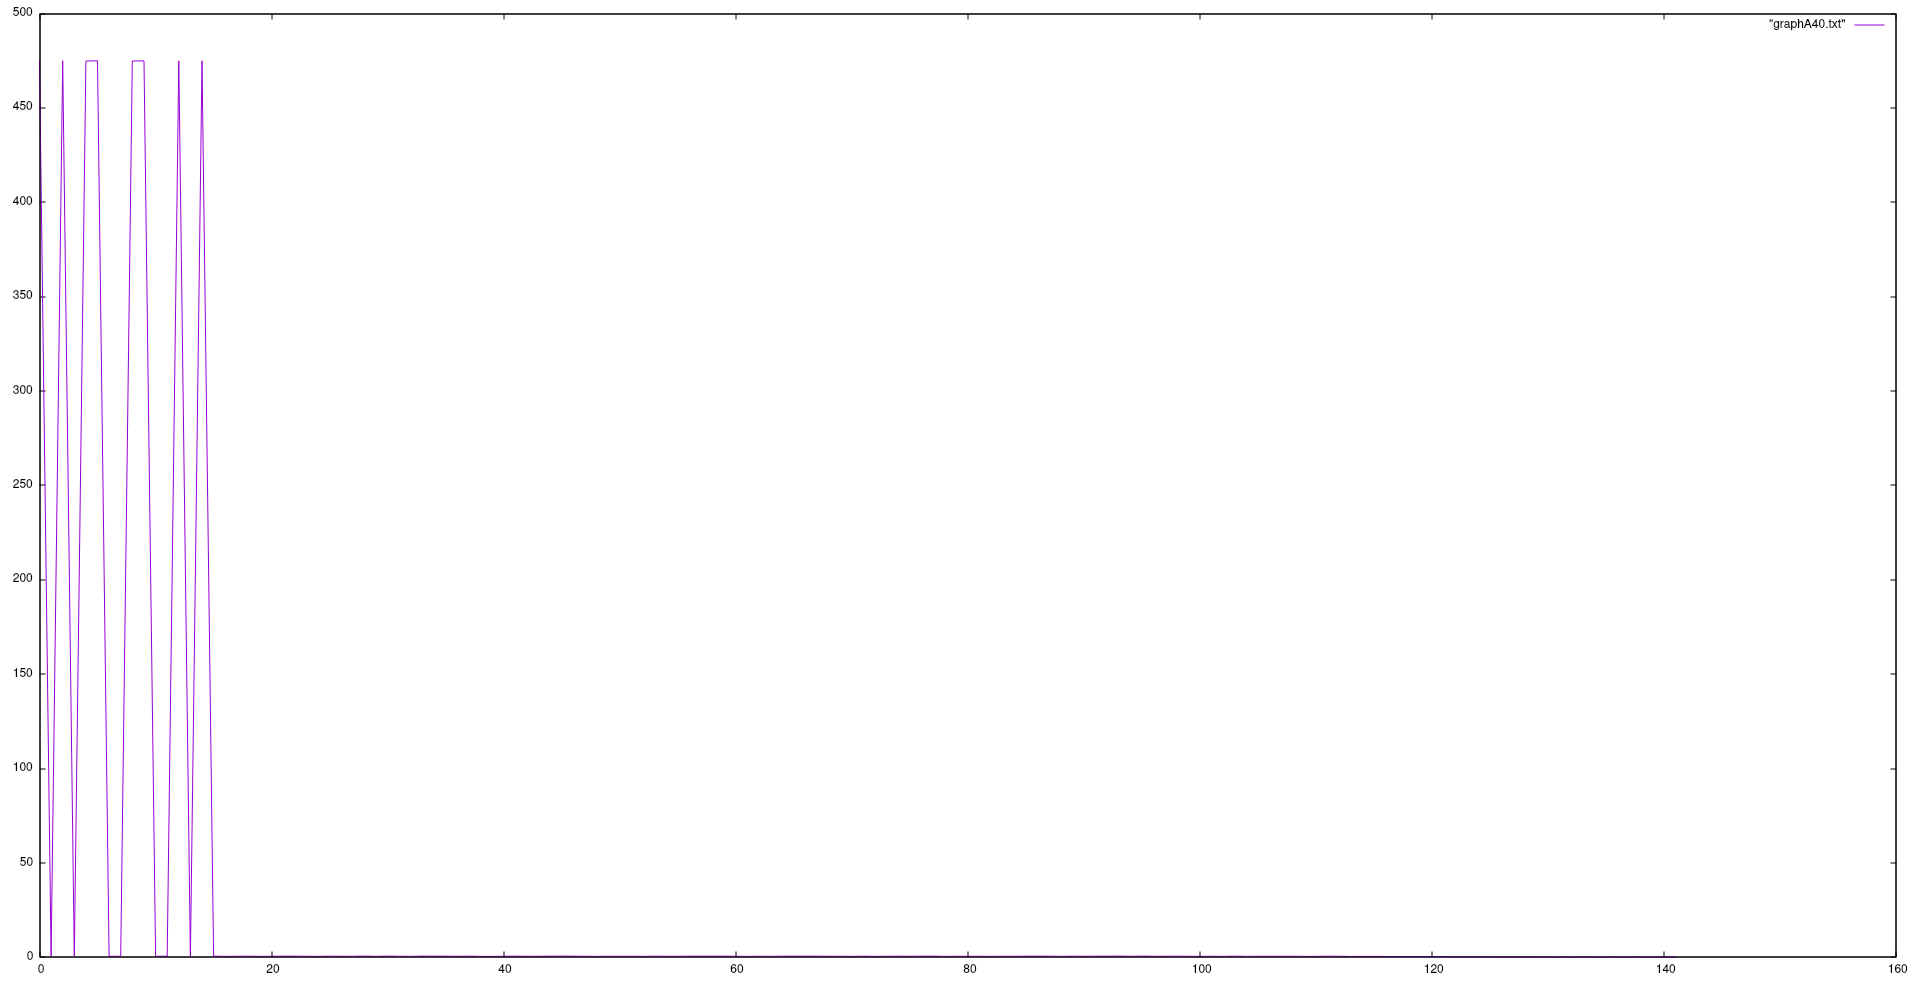
\includegraphics[scale=0.35]{A40}
    \caption{(A-40) Mejor solución: 0.224633} 
  \end{figure}
  \begin{figure}[!h]
    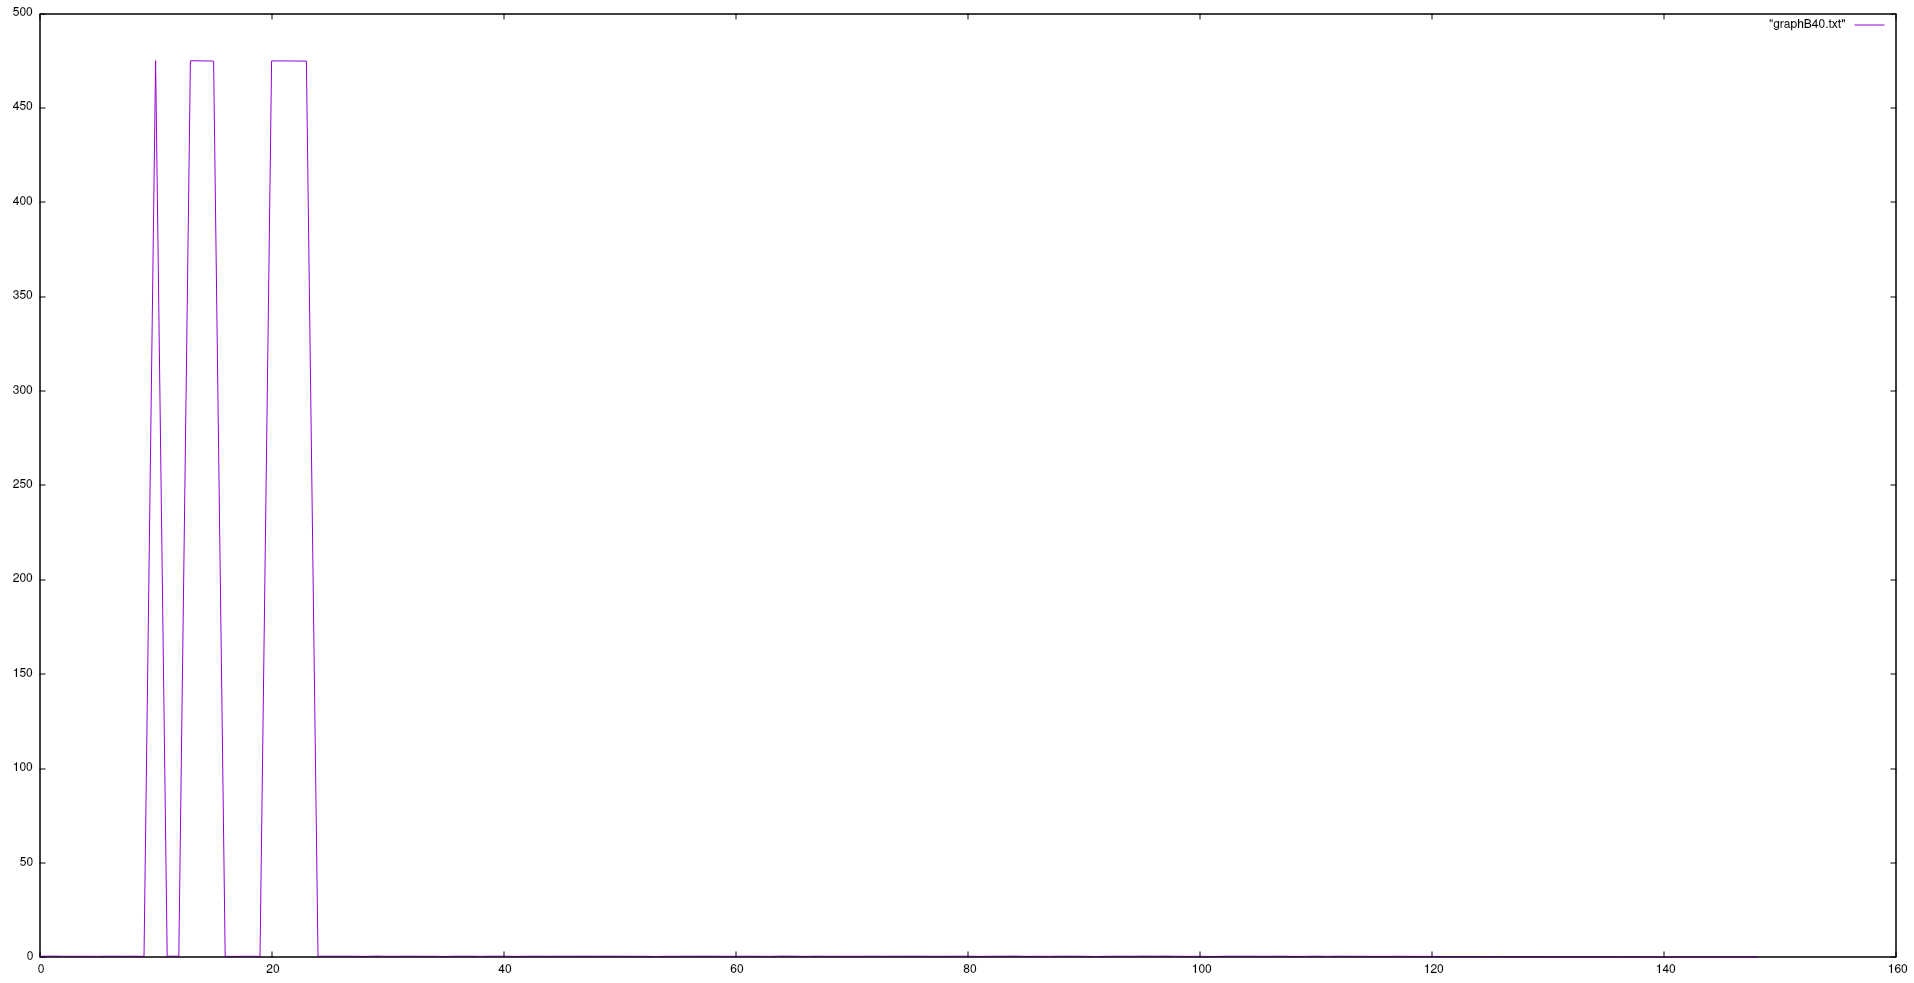
\includegraphics[scale=0.35]{B40}
    \caption{(B-40) Mejor solución: 0.217518} 
  \end{figure}
  \begin{figure}[!h]
    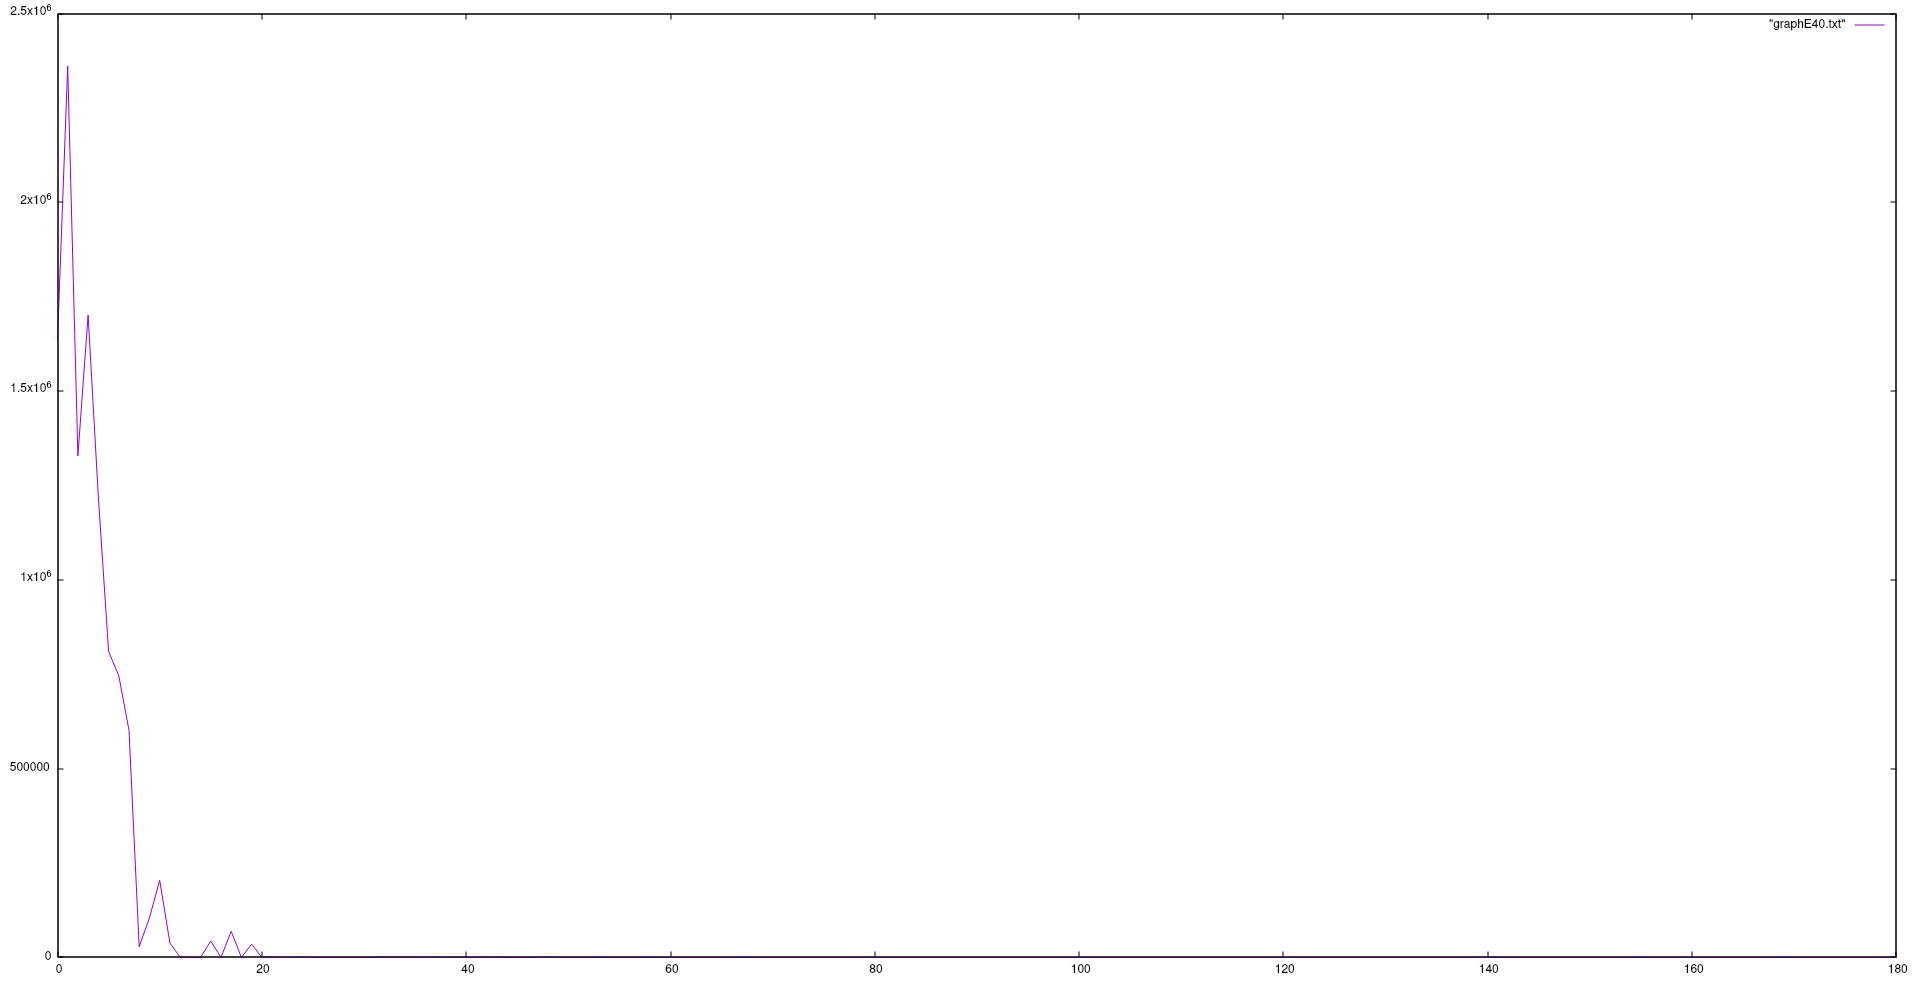
\includegraphics[scale=0.35]{E40}
    \caption{(E-40) Mejor solución: 0.217518} 
  \end{figure}
  \begin{figure}[!h]
    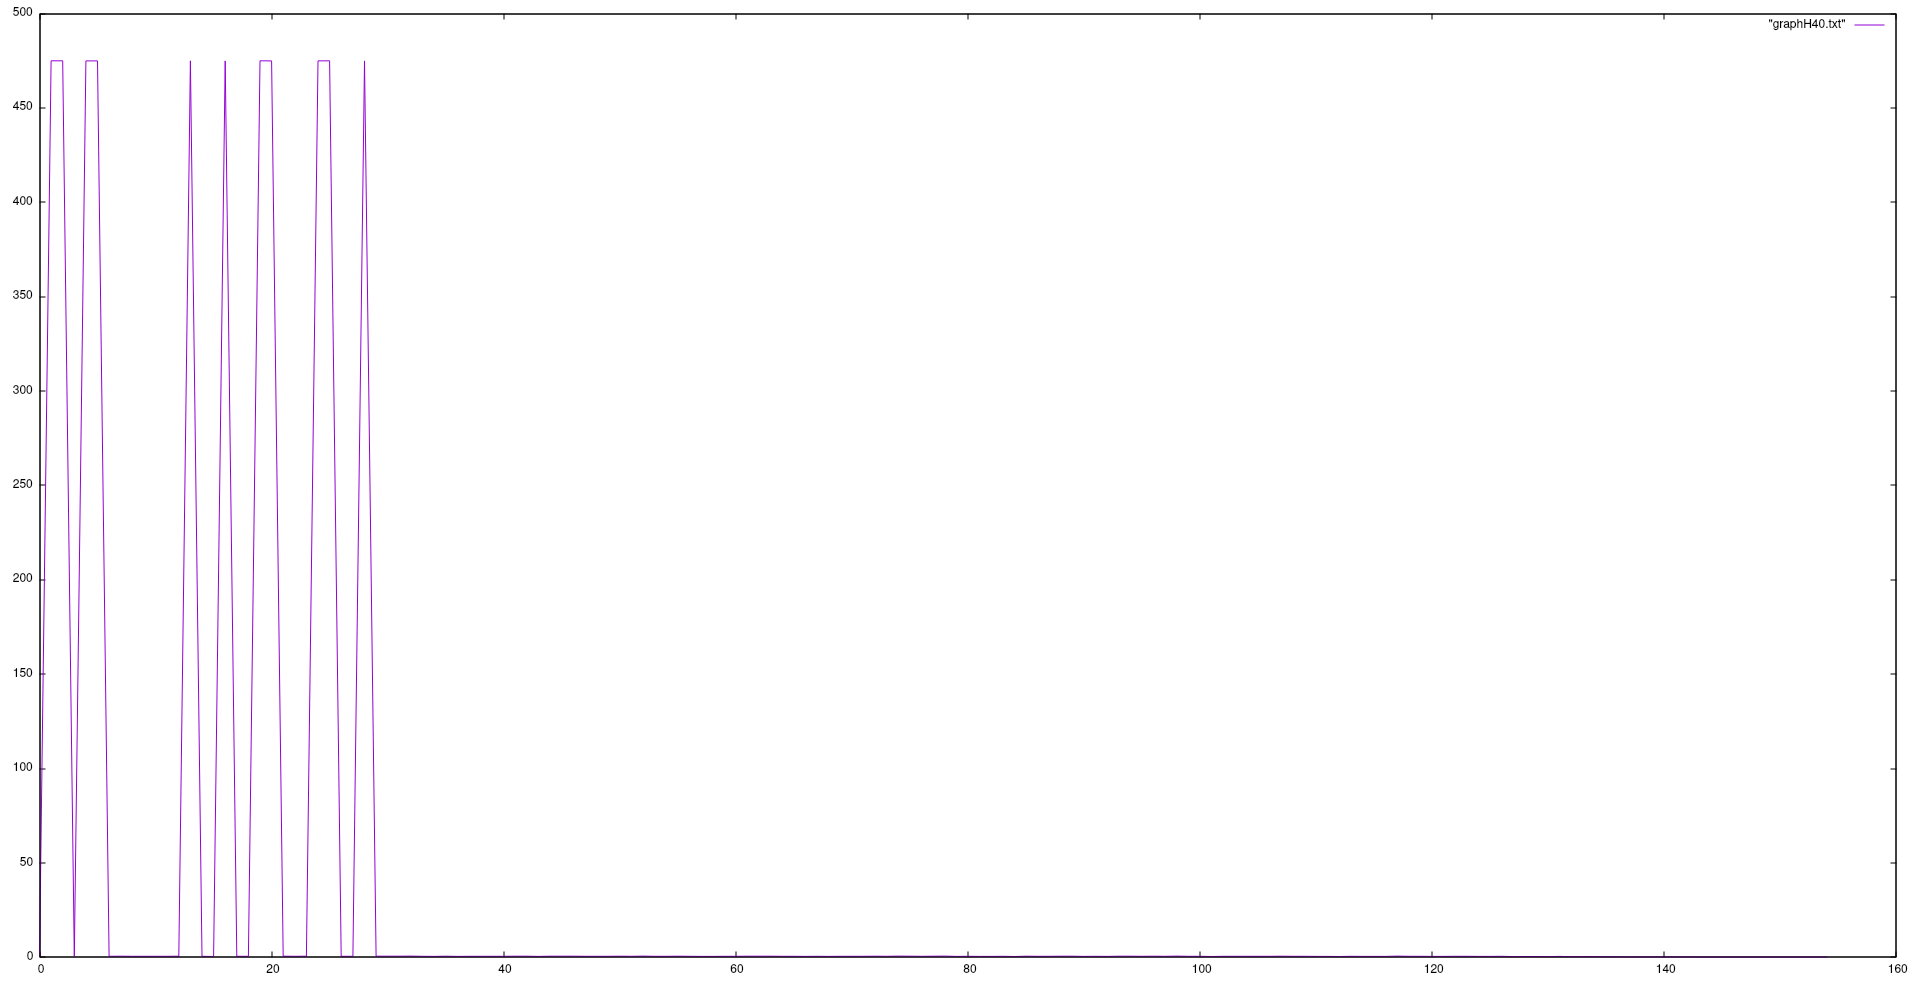
\includegraphics[scale=0.35]{H40}
    \caption{(H-40) Mejor solución: 0.222834} 
  \end{figure}
  \begin{figure}[!h]
    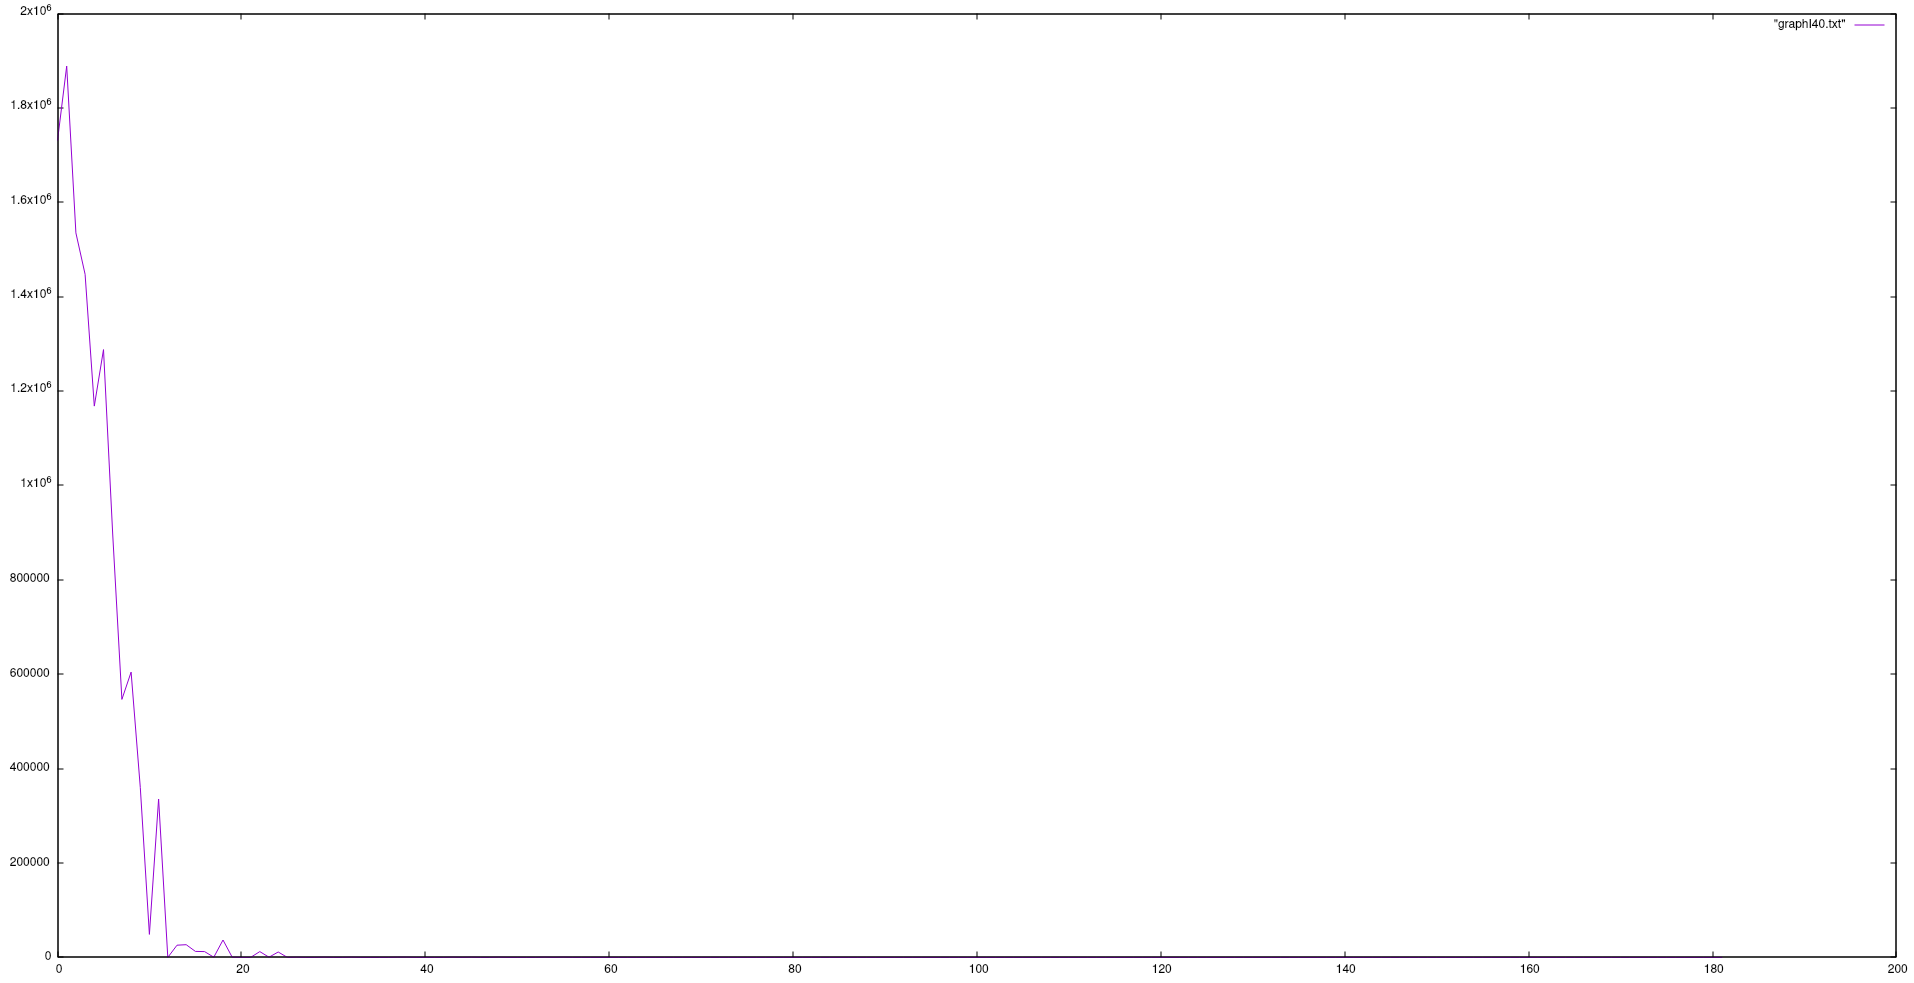
\includegraphics[scale=0.35]{I40}
    \caption{(I-40) Mejor solución: 0.217518} 
  \end{figure}

  \clearpage

  Y ahora presentando para el conjunto de 150 
  ciudades:

  \begin{figure}[!h]
    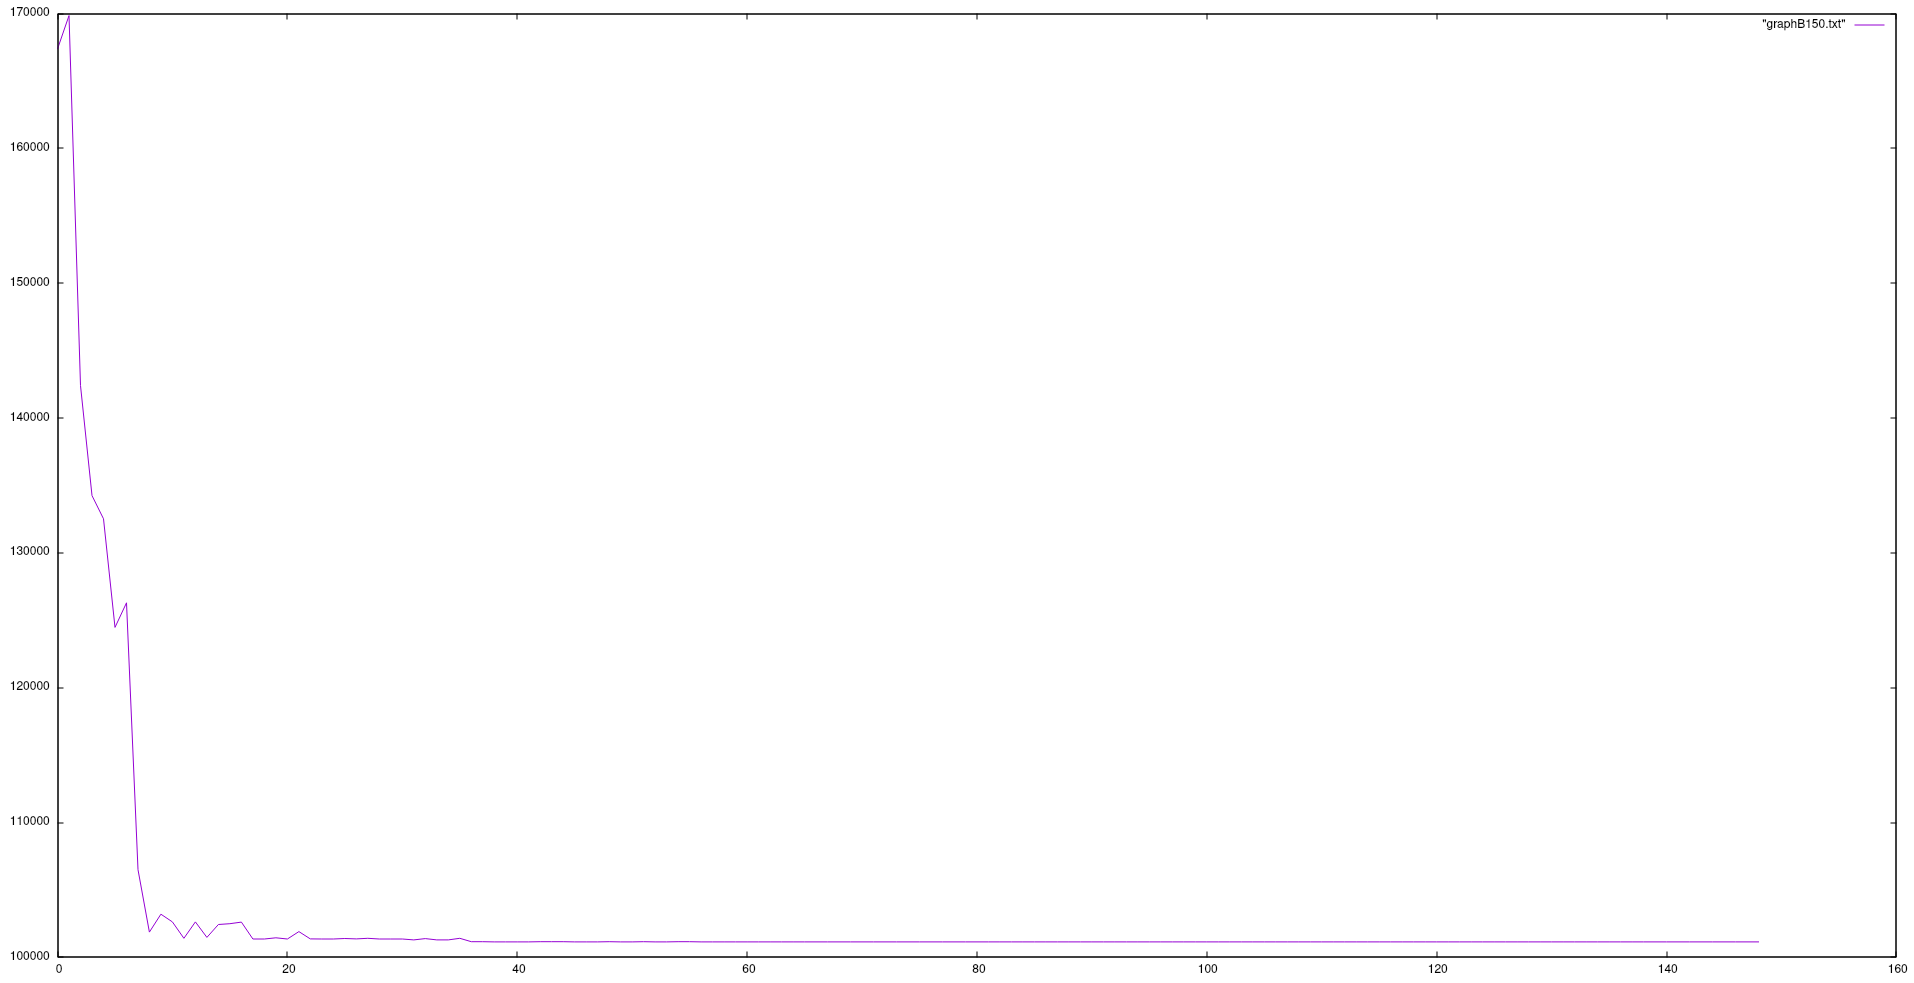
\includegraphics[scale=0.35]{B150}
    \caption{(B-150) Mejor solución: 101149.167010} 
  \end{figure}
  \begin{figure}[!h]
    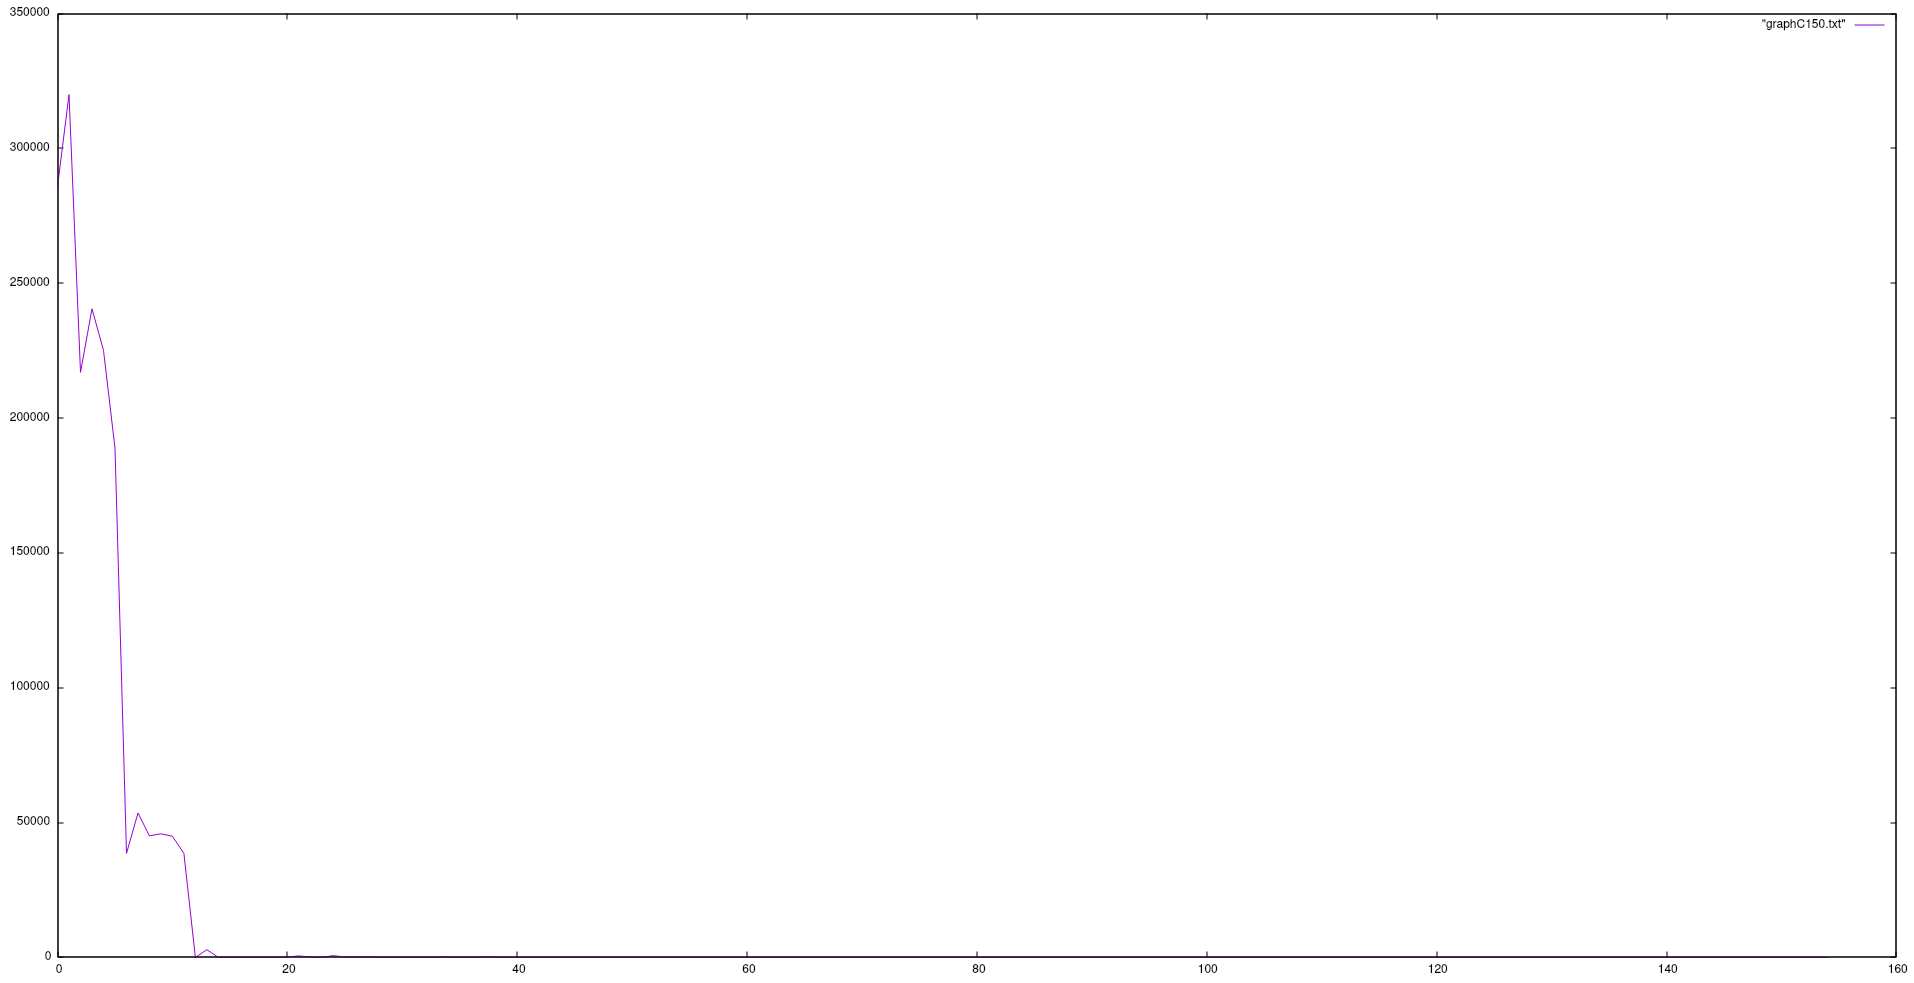
\includegraphics[scale=0.35]{C150}
    \caption{(C-150) Mejor solución: 0.209159} 
  \end{figure}
  \begin{figure}[!h]
    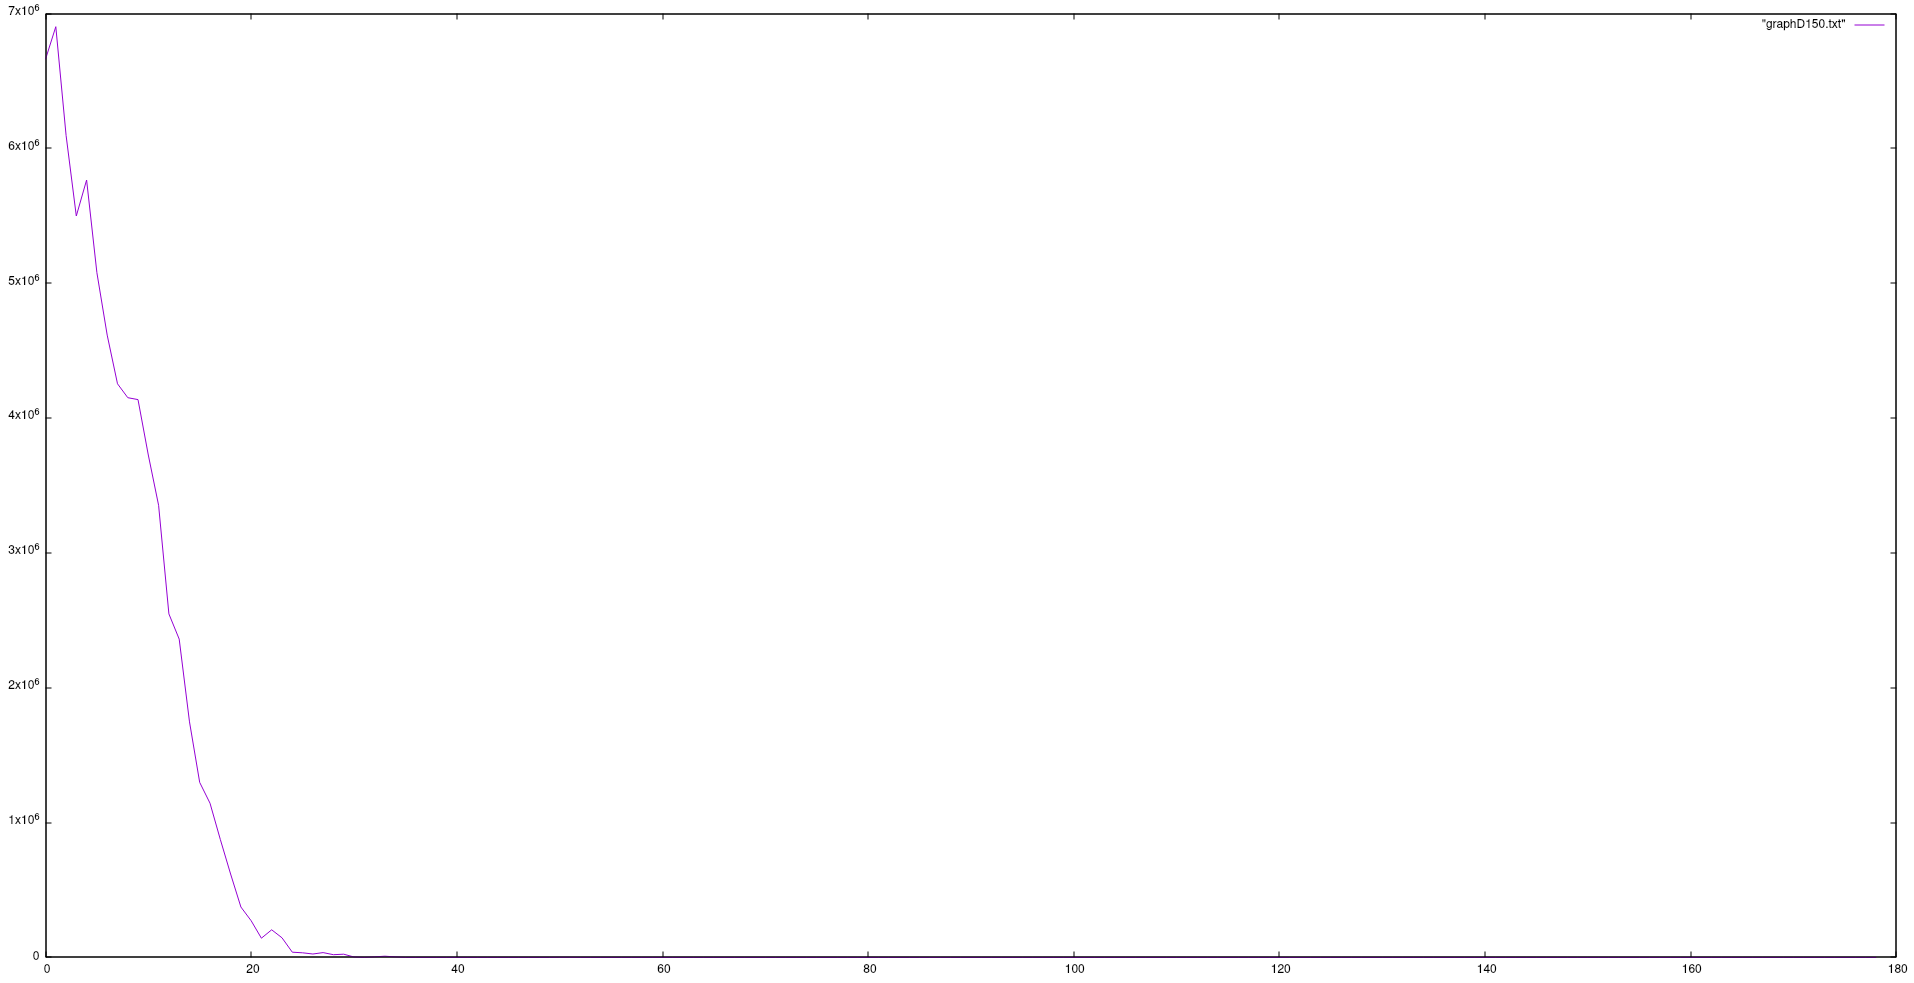
\includegraphics[scale=0.35]{D150}
    \caption{(D-150) Mejor solución: 0.175001} 
  \end{figure}
  \begin{figure}[!h]
    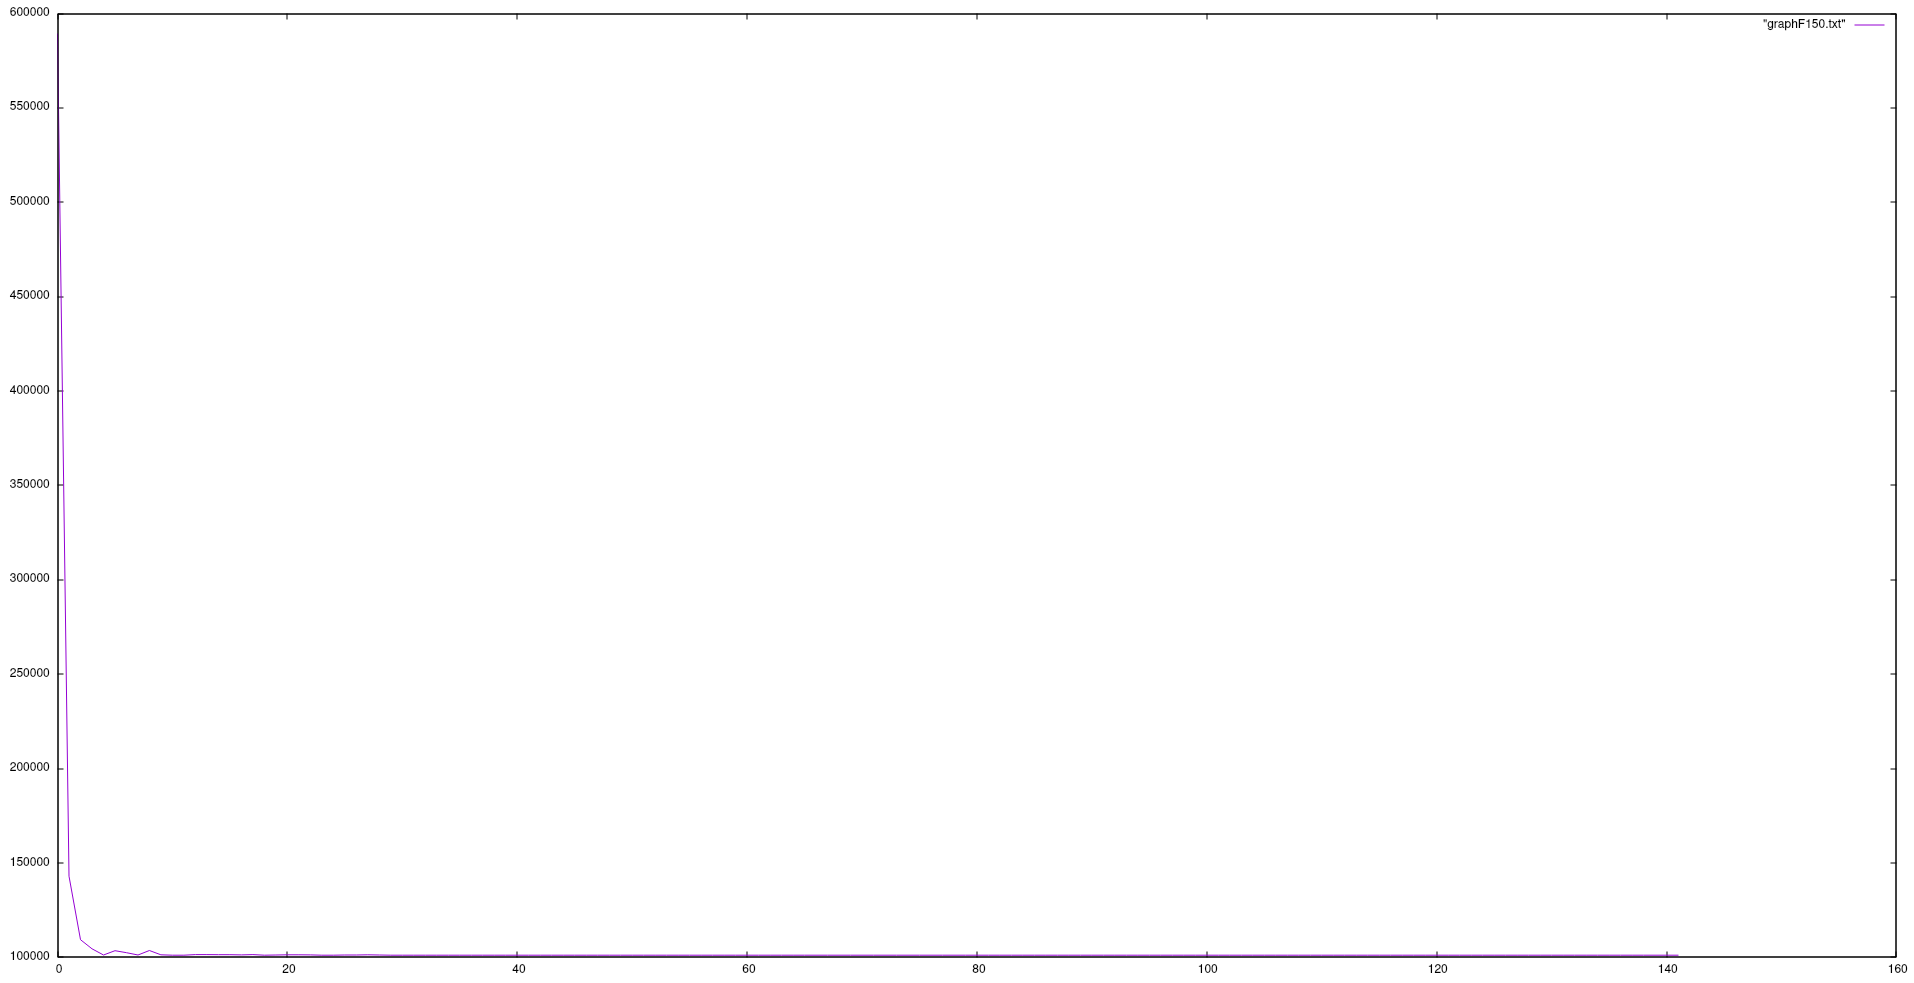
\includegraphics[scale=0.35]{F150}
    \caption{(F-150) Mejor solución: 101149.148309} 
  \end{figure}
  \begin{figure}[!h]
    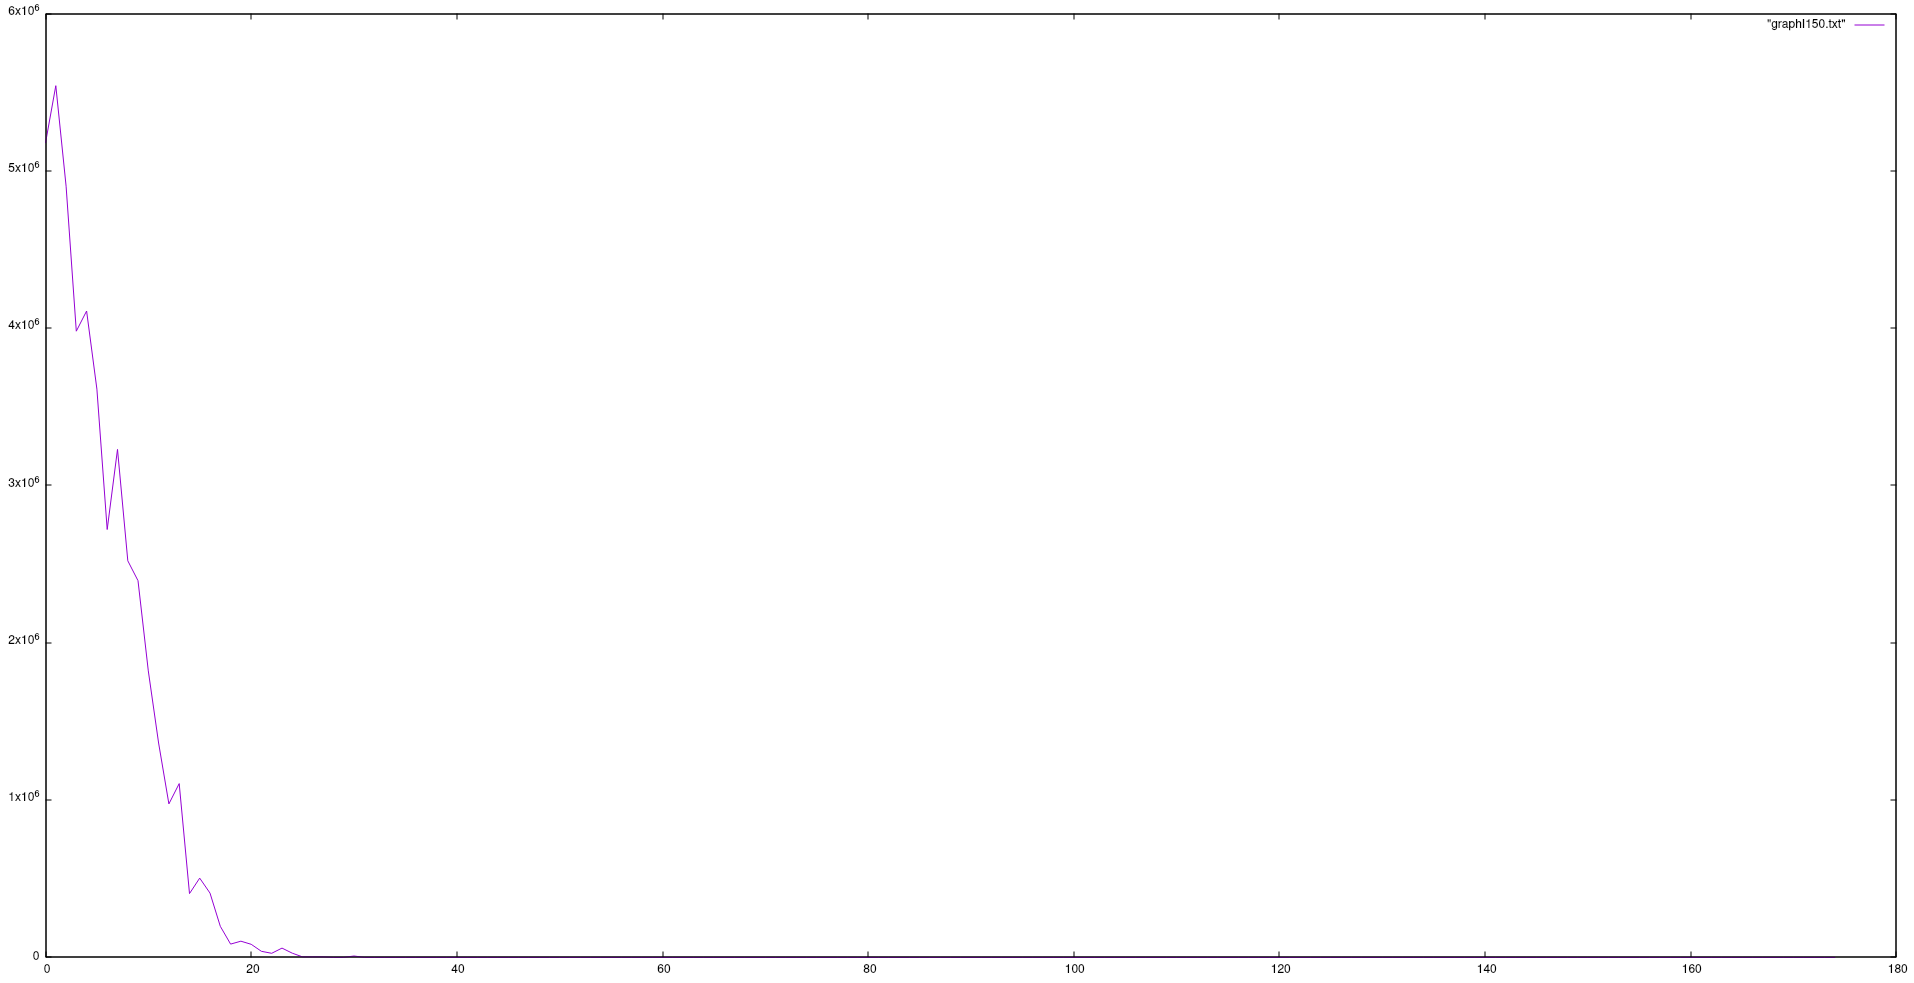
\includegraphics[scale=0.35]{I150}
    \caption{(I-150) Mejor solución: 0.184304} 
  \end{figure}
  \begin{figure}[!h]
    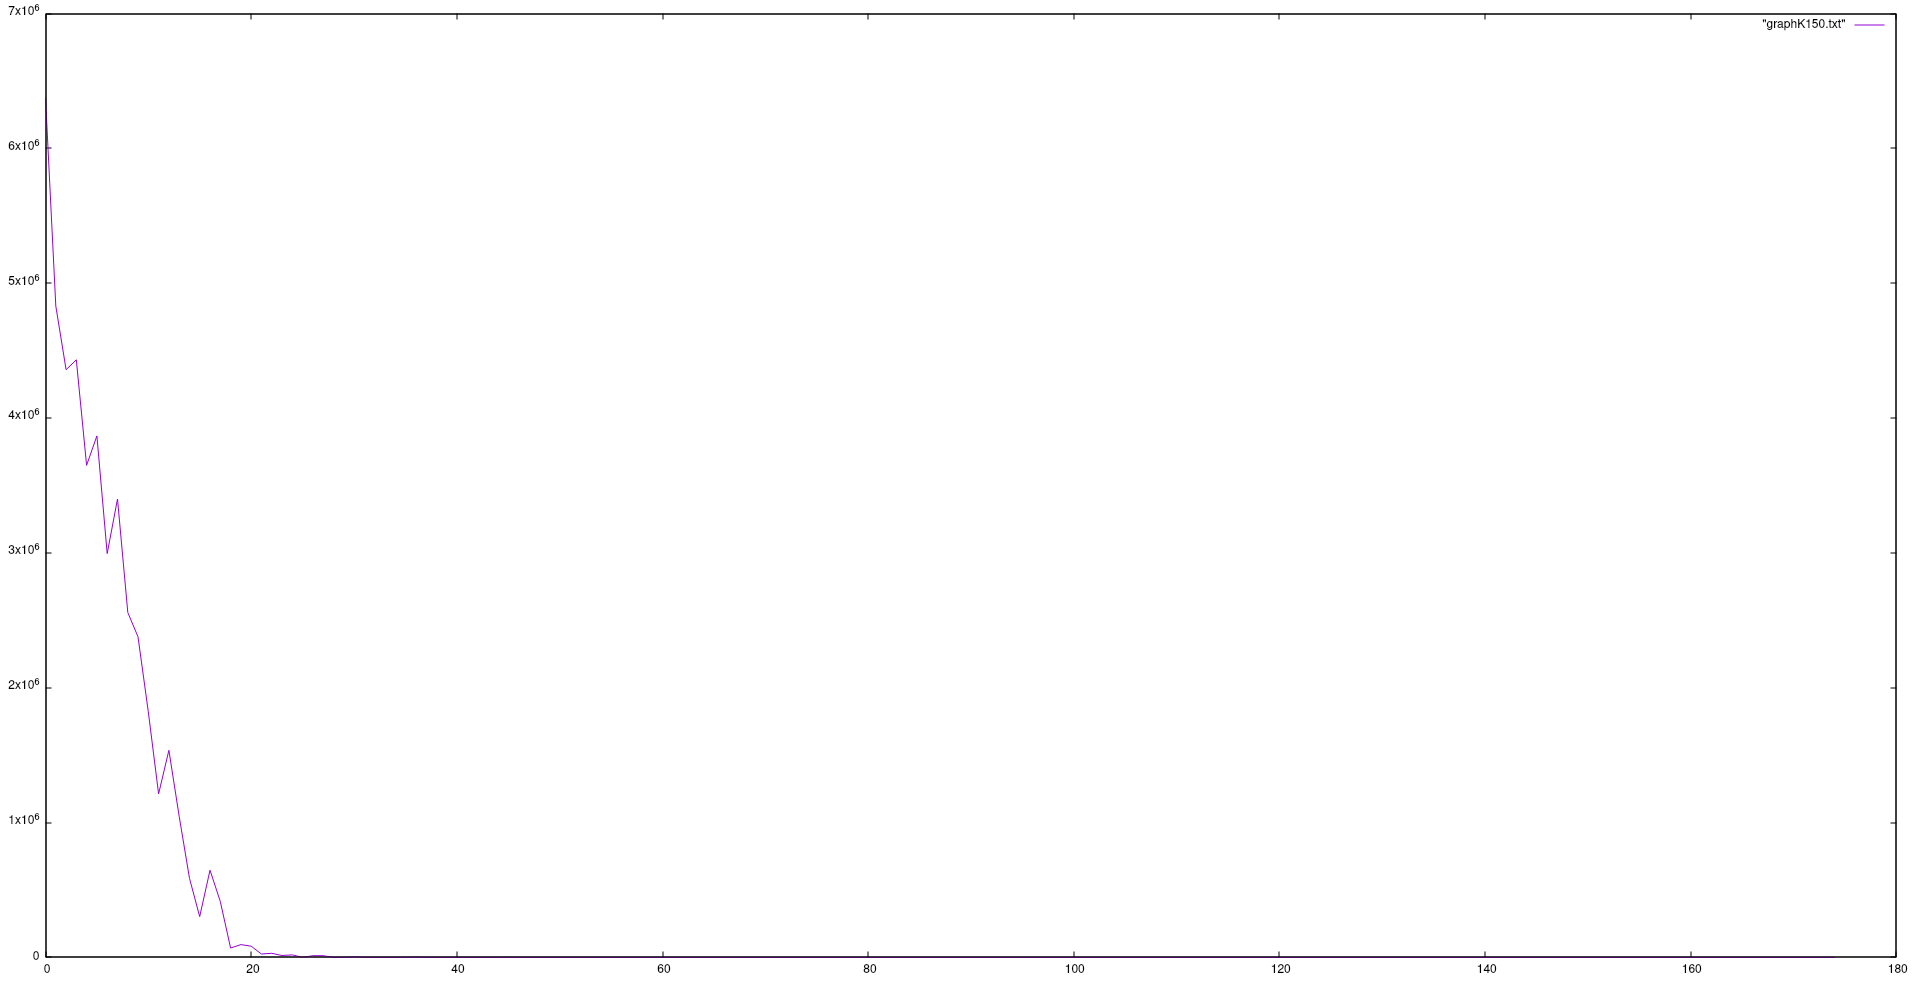
\includegraphics[scale=0.35]{K150}
    \caption{(K-150) Mejor solución: 0.160616} 
  \end{figure}
  \begin{figure}[!h]
    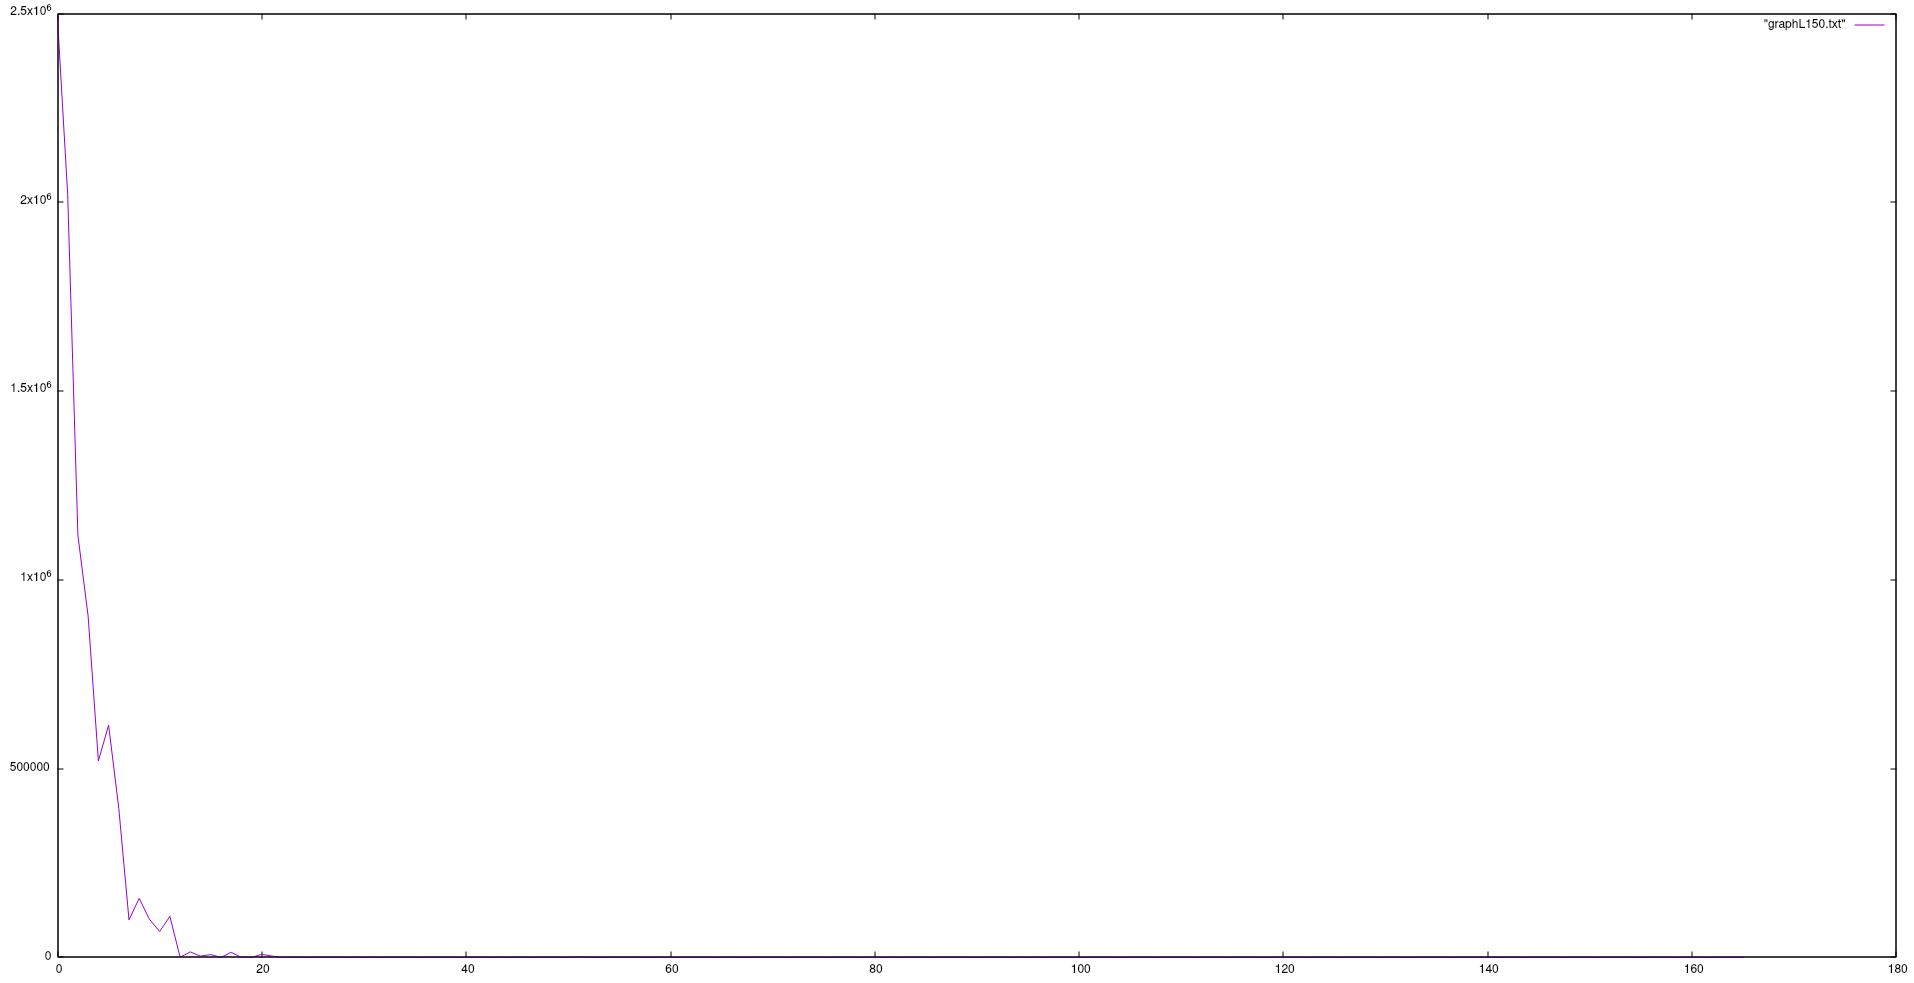
\includegraphics[scale=0.35]{L150}
    \caption{(L-150) Mejor solución: 0.162978} 
  \end{figure}

  \clearpage 

  \section{Discusión} \label{discussion}
  De todos los experimentos que se hicieron, 
  algo importante que se puede es que la temperatura
  y el tamaño del lote ($L$) sí terminan afectando 
  bastante el rendimiento de la heurística. 

  Los primeros experimentos se realizaron fueron con un 
  lote de tamaño 3000, y como esta cantidad es mucho mayor
  que el cuadrado de 40, entonces parece ser que la 
  huerística casi siempre (sin importar la temperatura)
  era capaz de regresar soluciones factibles. Por otro 
  lado, cuando tenemos 150 ciudades, es muy común 
  que nuestra heurística regrese muy malas soluciones, 
  esto lo podemos ver en la categoría A, B, F y G; la 
  razón por la que creemos que ocurre esto es porque 
  (además de que la temperatura no es lo suficientemente
  grande) el tamaño del lote es muy pequeño a comparación
  del cuadrado de 150.

  Ahora, la temperatura nos indice qué tanto va a estar
  ``buscando'' una solución. En el caso de las 40 ciudades
  para que temperaturas que estén entre 3000 y 12000 
  son bastante buenas para encontrar soluciones; sin 
  embargo, hay una mayor probabilidad de alcanzar una 
  solución muy cercana al \tit{óptimo} utilizando la 
  temperatura inicial dado un porcentaje de aceptación.
  Para 150 ciudades, es claro que temperaturas de 
  3000 o 6000 no son suficientes para poder encontrar
  soluciones factibles, no es hasta 12000 que empezamos 
  a tener como resultados soluciones factibles pero no 
  asegura que todas sean factibles (como se 
  puede ver en C); sin embargo, al igual que en el caso de 
  40 ciudades, con las temperaturas dadas por un porcentaje 
  de aceptación se obtienen resultados relativamente 
  bastante diferentes a comparación de los obtenidos 
  fijando una temperatura.
  
  En vista de lo anterior, se decidió hacer una prueba más 
  con el conjunto de 150 ciudades tomando las temperaturas 
  obtenidas con un porcentaje de aceptación y con un lote 
  de mayor tamaño, exactamente $\binom{150}{2}$. Los 
  resultados fueron los que se esperaban, soluciones
  cuyo costo esta \tit{relativamente} más cerca del 
  óptimo comparándolo con cualquiera de las antiguas 
  categorías; confirmando una vez más que el tamaño 
  del lote sí afecta directamente al rendimiento de la 
  huerística.

  Y gracias a las gráficas podemos qué tan rápido se 
  acerca la heurística a un mínimo local. Casos como en 
  F-150 o L-150 es fácil ver que la heurística se 
  atasca rápidamente en un mínimo local, en el caso de 
  F este mínimo resulta ser muy malo mientras que en L
  resulta ser muy bueno. En casos como A-40, B-40 y
  H-40, es muy común ver que gracias a la temperatura 
  la heurística es capaz de salir de estos mínimos locales
  para poder encontrar un mejor mínimo local; cosa que 
  por ejemplo con el conjunto de 150 ciudades casi no ocurre,
  siempre nos terminamos moviendo poco a poco sobre un 
  mismo mínimo local.

  \section{Conclusión} \label{conclusion}
  La heurística de aceptación por umbrales resulta ser 
  una muy buena alternativa para poder resolver 
  el problema del agente viajero, la única desventaja 
  de esta aproximación es que no es tan sencillo como 
  solo programar los algoritmos necesarios y listo; 
  se necesita experimentar con el tamaño del lote y con 
  la temperatura para ser capaces de conseguir, no 
  solo buenos resultados, sino resultados muy cercanos 
  al óptimo. Sin embargo, parece ser que este tipo 
  de valores que hay que buscar que nuestra heurística 
  funcione \tit{bastante} bien sólo se consiguen 
  a prueba y error.

\end{document}
